\documentclass[a4paper,11pt]{article}
\usepackage[margin=1in]{geometry}
\usepackage[T1]{fontenc}
\usepackage{lmodern}
\usepackage{amsmath,amssymb,amsthm,graphicx,booktabs}
\usepackage[hidelinks]{hyperref}
\hypersetup{pdftitle={Observable Certificates and Exact Termination in Backtracking Frank-Wolfe},pdfauthor={Yaroslav P. Lyakhov and Stepan A. Suvorov}}
\newtheorem{theorem}{Theorem}[section]
\newtheorem{lemma}[theorem]{Lemma}
\newtheorem{proposition}[theorem]{Proposition}
\newtheorem{corollary}[theorem]{Corollary}
\newcommand{\norm}[1]{\left\|#1\right\|}
\newcommand{\inner}[2]{\left\langle#1,#2\right\rangle}
\newcommand{\R}{\mathbb R}
\newcommand{\ceil}[1]{\left\lceil#1\right\rceil}
\DeclareMathOperator{\artanh}{artanh}
\title{Observable Certificates and Exact Termination\\in Backtracking Frank--Wolfe}
\author{Yaroslav P. Lyakhov \and Stepan A. Suvorov}
\date{1 November 2026}
\begin{document}
\maketitle
\begin{abstract}
We study observable stopping and exact termination in backtracking
Frank--Wolfe methods. For a convex objective with Lipschitz gradient on a
polytope whose entire solution set is an exposed face, ordinary quadratic
backtracking satisfies $G_k/(f(x_k)-f_Q^*)\to1$ along every infinite
nonterminal trajectory. A transfer argument for normalized atom weights
bounds the total number of exceptions and yields logarithmic local
complexity for an accumulated tangent certificate. The result concerns
algorithm trajectories: arbitrary near-optimal points need not satisfy
the same ratio, and an explicit convex $C^2$ example takes half-steps
forever. Endpoint Armijo probes at any predetermined unbounded sequence
of indices restore finite exact termination. For the function-dependent
Hessian model $H_0+H_1(f-f_Q^*)$, we also give separated certificate and
trial-evaluation bounds, a sharp pointwise gap envelope, and finite
away-step termination when $H_0=0$. An integrated curvature profile
provides a safe optimal-vertex test with deterministic gradient and
linear-oracle errors, provided a runner-up margin is certified and its
cost is counted separately. Exact example checks illustrate termination;
count-data controls measure the cost of unsuccessful probes outside the
solution-face assumptions. The results concern exact-oracle mechanisms
and do not establish universal practical speedup or minimax complexity.
\end{abstract}

\section{Introduction}
Frank--Wolfe (FW) replaces projections with linear minimization oracles~\cite{braun}.
Backtracking makes its quadratic step model usable without a prescribed
curvature constant, but a small primal error need not be visible to an
observable stopping certificate. This paper asks when FW can certify
progress, and when a certificate can lead to exact termination.

We first study ordinary FW on a polytope whose entire minimizing set is
a full exposed face. Assume that $f$ is convex and continuously
differentiable on a neighborhood of $Q$, its gradient is Lipschitz on
all of $Q$, and the atom oracle is exact. Theorem~\ref{face:ratio}
proves that along every infinite nonterminal trajectory, the FW gap
divided by primal suboptimality tends to one. A normalized-atom-weight
argument bounds the total number of exceptional updates and yields the
local observable-certificate complexity in Corollary~\ref{face:local}.
This is a trajectory statement; it does not assert the same ratio for
every near-optimal feasible point. Corollary~\ref{face:endpoint} shows
that sparse endpoint probes can force exact termination. An explicit
$C^2$ example shows why the probes matter: ordinary backtracking can
continue taking half-steps forever.

A complementary analysis concerns the constrained
loss-dependent Hessian bound
\[
 \|\nabla^2 f(x)\|\le H_0+H_1\bigl(f(x)-f_Q^*\bigr),
 \qquad x\in Q.
\]
This condition and its function-dependent-smoothness context are
previously studied~\cite{warmup,liuwarmup,kale,caoselfbound,lobanov}. Under it,
Theorem~\ref{thm:fw} bounds the updates and all rejected function trials
needed by ordinary backtracking to reach its observable certificate. The
update bound separates the $H_0/\varepsilon$ and
$H_1\log(1/\varepsilon)$ contributions and includes the initial
estimate. Its lag potential controls curvature estimates that remain
large as the certificate falls; the method and full-region LMO are
unchanged. Theorem~\ref{lem:bridge} gives the sharp pointwise FW-gap
envelope, attained by one-dimensional objectives. For away-step FW,
Theorem~\ref{thm:afw} gives the corresponding convex bound, while
Theorem~\ref{thm:geometric} gives logarithmic certificate accuracy under
an additional geometric gap inequality. At $H_0=0$,
Proposition~\ref{prop:zeroface} shows that the full solution set is an
exposed face with a common gradient, and Theorem~\ref{thm:zerofinite}
proves finite exact termination of backtracking AFW without that
additional inequality. The finite identification mechanism uses
established AFW results~\cite{bomze,garber}; we do not claim a new AFW
algorithm or general identification theory.

A further certificate uses curvature along a segment rather than a
single worst-case bound. Propositions~\ref{vertex:radius} and
\ref{vertex:certificate} give an integrated-curvature gradient radius
and a verifiable optimal-vertex test with deterministic oracle errors.
The test requires a certified runner-up margin. It establishes
certificate validity, not a complexity guarantee for a noisy method.
Safe-screening methods for convex and generalized conditional-gradient
problems provide related certificate context~\cite{raj,sunbach}.

\paragraph{Related work.}
Harks~\cite[Theorem 1 and Corollary 3]{harks} proves last-iterate
distance and gap rates for FW on monotone variational inequalities,
assuming Jacobian coercivity along the exposed face at a unique solution
and using prescribed reciprocal-step schedules. Our face result instead
allows a full, possibly non-singleton minimizing face and assumes only a
Lipschitz gradient; it bounds a trajectory-wise gap-to-objective ratio
and the local certificate cost under ordinary backtracking. Harks's
open-loop rates do not give the endpoint-probe stopping result.

Vyguzov and Stonyakin~\cite{vyguzov} analyze FW with
$\|\nabla^2 f(x)\|\le L_0+L_1\|\nabla f(x)\|$ and an adaptive step
rule. Their curvature depends on gradient norm, whereas ours depends on
loss suboptimality. On compact $Q$, convexity gives
$f-f_Q^*\le D\|\nabla f\|$, but replacing this by a global maximum
gradient does not retain our separated dependence. Oikonomou and Loizou
derive a related whole-space self-bounding inequality by ray comparison
\cite[Lemma B.7, Eq.~(30)]{oikonomouloizou}; that auxiliary inequality
is not a contribution claimed here.

Backtracking trial counts, Fenchel dual certificates, and linear AFW
convergence are already established by Pedregosa et al.
\cite[Theorems 1, 3, and 4]{pedregosa}. Our scalar lower-bound maximum
is distinct from their averaged-gradient Fenchel dual. Computable
tangent bounds are also classical~\cite[Method 1]{freundgrigas};
optimistic and primal--dual short steps explicitly optimize gaps under
global smoothness~\cite[Proposition 4.1]{beyondshort}. Appendix
\ref{app:comparison} discusses these and other adaptive, screening, and
active-set comparisons. We make no minimax-optimality, universal
speedup, or absolute-priority claim. The experiments isolate
initialization, active-face geometry, and certificate cost; the
cache-controlled endpoint study found no accepted probes or practical
improvement on tasks whose optima are not vertices.

\section{Ordinary backtracking and a computable certificate}
\label{sec:model}
Let $Q\subset\R^d$ be nonempty, compact and convex, with diameter
$D>0$. Let $f$ be convex and $C^2$ on a neighborhood of $Q$,
$f_Q^*=\min_Q f$, and $\delta(x)=f(x)-f_Q^*$. Assume
\begin{equation}\label{eq:curvature}
 \norm{\nabla^2f(z)}_2\le H_0+H_1\delta(z),\qquad z\in Q,
 \quad H_0,H_1\ge0.
\end{equation}
The reference value in this assumption is the constrained optimum.
A bound relative to a smaller unconstrained infimum does not imply the
same constrained bound without modifying $H_0$.
If $D=0$ the only feasible point solves the problem.

At a source $x_k$, obtain an exact linear minimization oracle (LMO),
and form the FW gap and accumulated certificate:
\begin{align}
 s_k&\in\arg\min_{v\in Q}\inner{\nabla f(x_k)}{v},\quad
 G_k=\inner{\nabla f(x_k)}{x_k-s_k},\label{eq:gap}\\
 \ell_k&=\max_{0\le i\le k}\{f(x_i)-G_i\},\quad
 U_k=f(x_k)-\ell_k.\label{eq:certificate}
\end{align}
Convexity gives $0\le\delta_k\le U_k\le G_k$. A valid known lower
bound can be included in $\ell_k$, but is not required. A zero gap
certifies optimality. We stop at $U_k\le\varepsilon$.
The best-so-far tangent construction is classical
\cite[Method 1, maximization convention]{freundgrigas}; the new
analysis concerns its curvature-dependent cost, not the certificate itself.

\paragraph{The algorithm.}
Choose $M>0$ and set $L_{-1}=M$. At each nonterminal source, put
$d_k=s_k-x_k$, $q_k=\norm{d_k}$, and start with $L=L_{k-1}/2$.
Repeat
\begin{equation}\label{eq:btstep}
 \alpha=\min\{1,G_k/(Lq_k^2)\},\qquad
 f(x_k+\alpha d_k)\le f(x_k)-\alpha G_k
                         +\tfrac12L\alpha^2q_k^2
\end{equation}
until the inequality passes, doubling $L$ after each rejection.
Store $L_k=L$, update $x_{k+1}=x_k+\alpha d_k$, and reuse the accepted
value. Only trial function values are recomputed during the search.
This is the standard quadratic backtracking scheme~\cite{pedregosa}.
For $M$ fixed, the algorithm does not need $D,H_0,H_1$, or $f_Q^*$.
The optional $M=U_0/D^2$ uses a diameter bound and the first paid
function, gradient and LMO calls.

\begin{lemma}[Local acceptance]\label{lem:local}
For a feasible descent direction $d$ with $g=-\inner{\nabla f(x)}d>0$
and feasible cap $a_{\max}>0$, the test in~\eqref{eq:btstep} passes
at $\alpha=\min\{a_{\max},g/(L\norm d^2)\}$ whenever
$L\ge H_0+H_1\delta(x)$. Every accepted trial, regardless of this
sufficient threshold, satisfies
\begin{equation}\label{eq:acceptedprogress}
 f(x)-f(x+\alpha d)\ge\tfrac12\alpha g.
\end{equation}
Thus the search terminates and
\begin{equation}\label{eq:localenvelope}
 L_k\le\max\{L_{k-1}/2,\ 2(H_0+H_1\delta_k)\}.
\end{equation}
The assertion also allows $a_{\max}>1$.
\end{lemma}
\begin{proof}
Write $h(t)=f(x+td)-f(x)$ and $K=H_0+H_1\delta(x)$.
While $h\le0$, the Hessian bound gives $h''(t)\le K\norm d^2$.
Initially $h'(0)=-g<0$. If $K>0$, a first return to zero before
$\min\{a_{\max},2g/(K\norm d^2)\}$ contradicts
$h(t)\le-gt+K\norm d^2t^2/2<0$. The same integration proves
the quadratic upper bound through the prescribed trial; the zero-$K$
case follows with a linear upper model. Its curvature is at most $L$,
so the test passes. For any accepted trial,
$L\alpha\norm d^2\le g$, proving~\eqref{eq:acceptedprogress}.
If there is a rejection, the last rejected estimate is less than $K$,
so the accepted one is less than $2K$; otherwise it is $L_{k-1}/2$.
\end{proof}

Consequently $f_k$ and $U_k$ are nonincreasing. The analysis uses
curvature only on a descent segment, not a uniform upper model on
every segment point.

\begin{lemma}[Lag potential]\label{lem:lag}
Let source phase indices be nondecreasing in $\{0,\ldots,J-1\}$.
Let positive caps obey $C_j/2\le C_{j+1}\le C_j$.
Suppose an update with $L_k>C_j$ in its source phase must have
$L_k=L_{k-1}/2$. Then the number of such lag updates is at most
\[
 \ceil{\log_2\max\{1,M/C_0\}}+J-1.
\]
The statement applies to every prefix and allows initially skipped phases.
\end{lemma}
\begin{proof}
Before an update in phase $j$, use the nonnegative integer potential
\[
 p=\max\{0,\ceil{\log_2(L_{k-1}/C_j)}\}.
\]
A lag update reduces it by one; a non-lag update leaves zero potential
before a phase change. A forward jump of $m$ phases raises it by at
most $m$. Starting from virtual phase zero, all jumps, including an
initial jump, sum to at most $J-1$. Nonnegativity proves the count.
\end{proof}

\begin{theorem}[Observable stopping and total function cost]\label{thm:fw}
For $0<\varepsilon<U_0$, let
\[
 J=\ceil{\log_2(U_0/\varepsilon)},\qquad
 P=\ceil{\log_2\max\{1,MD^2/U_0\}}.
\]
Ordinary backtracking reaches $U_N\le\varepsilon$ within
\begin{equation}\label{eq:fwcount}
 N\le P+\ceil{(6+16H_1D^2)J+32H_0D^2/\varepsilon}
\end{equation}
updates. It uses $N+1$ gradients and LMOs, including the final check.
For its actual $N\ge1$, every function evaluation, including all
rejected trials, is counted in
\begin{equation}\label{eq:functioncount}
 N_f\le1+2N+\ceil{\log_2\max\{1,2(H_0+H_1U_0)/M\}}.
\end{equation}
For $N=0$, one function, gradient and LMO evaluation suffice.
These are exact-oracle and exact-arithmetic bounds.
\end{theorem}
\begin{proof}
Put $b_j=U_0/2^j$ and assign a nonterminal source to phase $j$ when
$b_j/2<U_k\le b_j$, for $j=0,\ldots,J-1$.
Use
\[
 C_j=\max\{2(H_0+H_1b_j),\ b_j/(2D^2)\}.
\]
The caps decrease by at most a factor two. By
Lemma~\ref{lem:local}, an accepted estimate above $C_j$ must be a
first-trial halving. Since $C_0\ge U_0/(2D^2)$,
Lemma~\ref{lem:lag} bounds lag updates by $P+J$.

For a non-lag update in phase $j$, $G_k\ge U_k>b_j/2$ and
$q_k\le D$ imply
\[
 f_k-f_{k+1}\ge p_j:=\min\{b_j/4,\ b_j^2/(8C_jD^2)\}.
\]
Every update decreases $f$, and the total decrease within the phase
is at most its initial suboptimality, hence at most $b_j$.
Thus its non-lag updates number at most
\[
 \lfloor b_j/p_j\rfloor+1
 \le5+16H_1D^2+16H_0D^2/b_j.
\]
Summing and using $\sum_{j<J}1/b_j<2/\varepsilon$ proves
\eqref{eq:fwcount}. This bounds every unfinished prefix, which also
establishes termination.

The local envelope and monotone $U$ give
$L_k\le\max\{M/2^{k+1},2(H_0+H_1U_0)\}$.
If $r_k$ denotes rejections, $L_k=2^{r_k-1}L_{k-1}$, so exactly
\[
 \sum_{k<N}(r_k+1)=2N+\log_2(L_{N-1}/M)
\]
trial values are computed. Add the initial value and use the envelope
to obtain~\eqref{eq:functioncount}. Accepted values are cached.
\end{proof}

The last identity is standard~\cite{pedregosa}. For $M=U_0/D^2$,
$P=0$, and the function-count overhead is independent of
$\varepsilon$. This normalization is optional for the order of the bound.

\begin{proposition}[Initialization is visible even for affine objectives]
\label{prop:init}
Let $Q=[-1,1]$, $f(x)=-cx$, $c>0$, $x_0=-1$, and $L_{-1}=M>0$.
For $0<\varepsilon<2c$, halving backtracking uses exactly
\[
 N=\ceil{\log_2\left(1+\frac Mc(1-\varepsilon/(2c))\right)}
\]
updates. Thus halving $U_0$ may require $\Theta(\log(M/c))$ updates.
\end{proposition}
\begin{proof}
Every test accepts its first trial: $L_k=M/2^{k+1}$,
$x_{k+1}=\min\{1,x_k+c/L_k\}$. The tangent lower bound is always
$-c$, so $x_N=\min\{1,-1+(2c/M)(2^N-1)\}$ and $U_N=c(1-x_N)$.
Solving the stopping inequality gives the formula.
\end{proof}
This lower bound concerns the specified halving rule, not arbitrary
first-order algorithms. With $M=U_0/D^2=c/2$ the first step solves it.

\paragraph{Comparison with a global bound.}
For $f(x)=\cosh(x)-1$ on $[-R,R]$, $H_0=H_1=1$, while a global
gradient-Lipschitz constant is $L_Q=\cosh R$. Starting at $R$ gives
$U_0=2R\sinh R$. For fixed tolerance and fixed $M$, our update bound
grows as $O(R^3+R^2/\varepsilon)$ as $R\to\infty$, rather than the
exponential $L_QD^2/\varepsilon$ term obtained by substituting
$H_0=L_Q,H_1=0$ in the same certificate theorem.
This compares upper bounds, not a runtime or oracle lower bound;
exact segment minimization solves this particular one-dimensional example
in one step. Appendix~\ref{app:explicit} gives further step comparisons.

\section{Away steps and geometric progress}
Let $Q=\operatorname{conv}(\mathcal A)$ for a finite atom set.
Maintain $x=\sum_{a\in S}\lambda_a a$ with positive weights summing
to one. Besides the full FW atom $s$, choose
$v\in\arg\max_{a\in S}\inner{\nabla f(x)}a$.
Use the larger-gap direction among $s-x$ and $x-v$, choosing FW on a
tie. Its gap $g$ satisfies $g\ge G\ge U$ and its norm is at most $D$.
The feasible cap is $1$ for FW and $\lambda_v/(1-\lambda_v)$ for
away; a singleton takes FW. Apply the same halving/doubling test with
$\alpha=\min\{a_{\max},g/(L\norm d^2)\}$.
This is standard away-step FW (AFW)~\cite{lacostejaggi,pedregosa}.
The certificate still uses the full FW gap. Active-set search is
additional work, separate from full LMO calls.

An away step at its cap removes an atom and is called a drop;
other steps are good. If $m$ good updates occur, drops number at most
the number of FW updates plus $|S_0|-1$, hence
\begin{equation}\label{eq:dropcount}
 N\le2m+|S_0|-1.
\end{equation}
This follows because FW adds at most one atom and a drop removes one,
while the active set remains nonempty. Full FW steps can remove more
atoms and only improve the bound.

\begin{theorem}[Convex AFW certificate bound]\label{thm:afw}
With $J,P$ as in Theorem~\ref{thm:fw}, AFW reaches
$U_N\le\varepsilon$ within
\[
 N\le2\left[P+\ceil{(6+16H_1D^2)J+32H_0D^2/\varepsilon}\right]
       +|S_0|-1.
\]
It uses $N+1$ gradients and full LMOs.
Its actual function-call count satisfies~\eqref{eq:functioncount}.
\end{theorem}
\begin{proof}
Use the caps and phase potential from Theorem~\ref{thm:fw}, counting
lag across all updates. On a good away step the quadratic minimizer
is not clipped, giving decrease $g^2/(2L\norm d^2)$.
A full FW step gives at least $g/2$; a nonfull FW step has the same
quadratic bound. Thus controlled good steps have the same lower
progress $p_j$ as in that theorem. Drops also decrease $f$, so the
phase budget still bounds the good steps by the ordinary FW count.
Apply~\eqref{eq:dropcount}. Lemma~\ref{lem:local}, the accepted-estimate
envelope and the trial-count identity remain valid across drops,
proving the function bound.
\end{proof}

\subsection{From primal progress to the observable threshold}
For geometric convergence assume the selected gap satisfies
\begin{equation}\label{eq:geometry}
 g_k^2\ge2\kappa\delta_k,\qquad\kappa>0.
\end{equation}
This is an extra hypothesis. For example strong convexity $\mu>0$
and pyramidal width $W$ give $\kappa=\mu W^2/4$.
Quadratic growth relative to a possibly non-singleton solution set,
$\delta(x)\ge(\gamma/2)\operatorname{dist}(x,X^*)^2$ on the initial
sublevel set, gives $\kappa=\gamma W^2/16$.
These are established polytope scaling implications;
Appendix~\ref{app:geometry} records the constants and
attribution~\cite{lacostejaggi,restartfw}.

Freezing curvature at the source gives the two-branch quadratic
envelope in Appendix~\ref{app:bridge}, by the established descent
inversion~\cite[Eq.~(15)]{lacoste2016}. Retaining its dependence on
the function along the segment gives the exact envelope for our class.

\begin{theorem}[Optimal pointwise FW-gap envelope]\label{lem:bridge}
Suppose $H_1>0$, and write $a=D\sqrt{H_1}$ and $c=H_0/H_1$.
At every feasible source,
\begin{equation}\label{eq:optimalbridge}
 U\le G\le E(\delta):=
 \begin{cases}
 D\sqrt{2H_0\delta+H_1\delta^2},&\delta\le c(\cosh a-1),\\
 a\delta\coth a+ac\tanh(a/2),&\delta>c(\cosh a-1).
 \end{cases}
\end{equation}
For every $D>0$, $H_0\ge0$, $H_1>0$ and $\delta>0$, a convex
$C^2$ objective on a one-dimensional interval of diameter $D$
attains equality. Thus no smaller bound depending only on these
four quantities is valid for this class.
The inverse envelope is
\begin{equation}\label{eq:threshold}
 \eta_\varepsilon=
 \begin{cases}
 \displaystyle\frac{(\varepsilon/D)^2}
 {H_0+\sqrt{H_0^2+H_1(\varepsilon/D)^2}},
       &\varepsilon\le ac\sinh a,\ H_0>0,\\[6pt]
 \displaystyle\frac{\varepsilon}{a}\tanh a-c(1-\operatorname{sech}a),
       &\text{otherwise}.
 \end{cases}
\end{equation}
Hence $\delta\le\eta_\varepsilon$ implies $U\le\varepsilon$.
For $H_1=0$, put $A=D^2H_0$: the limiting envelope is
$\sqrt{2A\delta}$ for $2\delta\le A$, and $\delta+A/2$ otherwise;
its inverse is $\varepsilon^2/(2A)$ for $\varepsilon\le A$,
and $\varepsilon-A/2$ otherwise. At $H_0=H_1=0$ these are
$E(\delta)=\delta$ and $\eta_\varepsilon=\varepsilon$.
\end{theorem}
\begin{proof}
Set $h(t)=f(x+t(s-x))-f_Q^*$ for $0\le t\le1$.
Then $h\ge0$, $h(0)=\delta$, $h'(0)=-G$, and
$h''\le D^2(H_0+H_1h)=a^2(h+c)$.
Variation of constants, whose kernel $\sinh(a(t-u))/a$ is
nonnegative for $u\le t$, gives
\[
 0\le h(t)\le(\delta+c)\cosh(at)-(G/a)\sinh(at)-c.
\]
Consequently, for every $0<t\le1$,
\[
 G\le a\frac{(\delta+c)\cosh(at)-c}{\sinh(at)}.
\]
For $c>0$ its derivative changes sign at
$\cosh(at)=1+\delta/c$. If this point lies in the segment,
the minimum is $a\sqrt{\delta(\delta+2c)}$; otherwise it is
the value at $t=1$. For $c=0$ the expression is decreasing
and its minimum is $a\delta\coth a$. These are~\eqref{eq:optimalbridge}.
The increasing branches meet at $\delta=c(\cosh a-1)$, where
$E=ac\sinh a$. Inversion gives~\eqref{eq:threshold}.
Appendix~\ref{app:bridge} constructs attaining objectives for both
branches, including convex $C^2$ extensions beyond the interval.
For $H_1=0$, integrate $h''\le D^2H_0$ and minimize
$\delta/t+D^2H_0t/2$ on $(0,1]$.
\end{proof}

The word ``optimal'' here concerns a pointwise inequality within the
specified function class, not oracle complexity or bibliographic priority.
At $H_0=0$ the relation is linear, $G\le a\coth(a)\delta$.
For fixed $H_0>0$ and small tolerance,
$\eta_\varepsilon=\Theta(\varepsilon^2)$; this exponent cannot be
removed in general: $f(x)=x^2/2$ on $[-1,1]$, at $x=t>0$, gives
$\delta=t^2/2$ and $G=t(1+t)$. At the first observation $U=G$.
This is not an iteration lower bound or a restriction on stronger
history-dependent certificates.

\begin{figure}[tb]
\centering
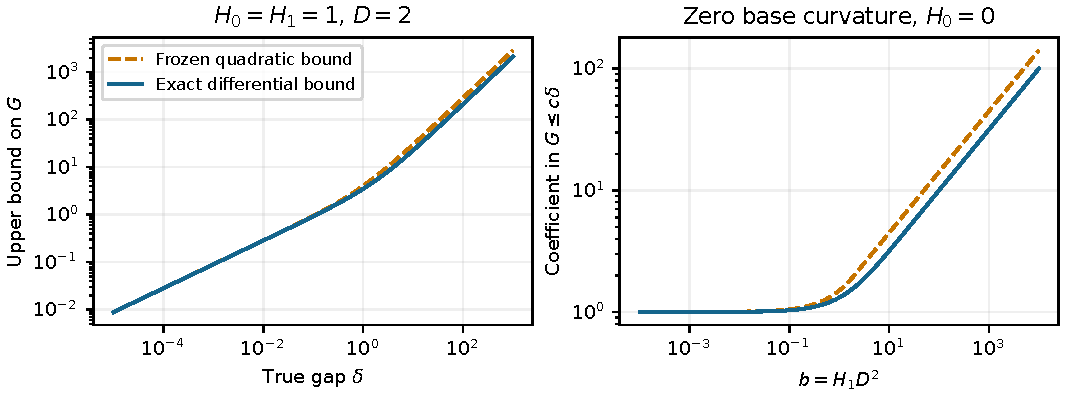
\includegraphics[width=\linewidth]{figures/gap_geometry.pdf}
\caption{Pointwise theoretical bounds. The differential envelope retains
the changing function value along the segment; the frozen quadratic
comparison is~\eqref{eq:sharpbridge}. At zero base curvature, the exact
linear coefficient is $\sqrt b\coth\sqrt b$. These are inequalities
over a function class, not optimization trajectories or timing results.}
\label{fig:geometry}
\end{figure}

\begin{theorem}[Geometric AFW certificate bound]\label{thm:geometric}
Assume $H_0+H_1>0$ and~\eqref{eq:geometry}. Set
\[
 J_*=\ceil{\log_2(U_0/\eta_\varepsilon)},\qquad
 P_*=\ceil{\log_2\max\{1,M/[2(H_0+H_1U_0)]\}}.
\]
For $0<\varepsilon<U_0$, the same algorithm reaches
$U_N\le\varepsilon$ within
\begin{equation}\label{eq:geometriccount}
 N\le2\ceil{P_*+(6+4H_0D^2/\kappa)J_*+8H_1D^2U_0/\kappa}
       +|S_0|-1.
\end{equation}
Equation~\eqref{eq:functioncount} remains valid. None of
$H_0,H_1,\kappa,f_Q^*$ is an algorithm input.
\end{theorem}
\begin{proof}
Analyze true-error phases $b_j/2<\delta_k\le b_j$ with
$b_j=U_0/2^j$, until $\delta\le\eta_\varepsilon$.
Their positive caps $C_j=2(H_0+H_1b_j)$ decrease by at most a factor
two. The initial true error may skip phases; Lemma~\ref{lem:lag}
still bounds lag updates by $P_*+J_*$.
On a controlled good step,
\[
 f_k-f_{k+1}\ge\delta_k\min\{1/2,\kappa/(C_jD^2)\}
 >\min\{b_j/4,\kappa b_j/(2C_jD^2)\}.
\]
For a full FW step use $g\ge G\ge\delta$; for a nonclipped step
use~\eqref{eq:geometry}. The phase budget $b_j$ permits at most
$5+4H_0D^2/\kappa+4H_1D^2b_j/\kappa$ controlled good updates.
Sum $\sum_{j<J_*}b_j<2U_0$, add lag updates and
apply~\eqref{eq:dropcount}. Theorem~\ref{lem:bridge} ensures the actual
certificate has passed by this point.
\end{proof}

For fixed problem and initialization the accuracy dependence is
logarithmic. The explicit $H_1$ phase cost is proportional to $U_0$;
$H_1$ also enters $J_*$ through~\eqref{eq:threshold}.
Both AFW bounds apply when the geometric hypothesis holds; the
initial $U_0/\kappa$ contribution means the geometric bound is not
uniformly tighter than the convex one.
One need not assume $H_0>0$: the caps are positive at positive phase
levels when $H_1>0$. A nonaffine example is $f=t+(\max\{t,0\})^3$,
$t=1/2-x$, on $[-1/2,1/2]$, with $H_0=0,H_1=6$ and
$\kappa=1/16$ (Appendix~\ref{app:bridge}). In fact $H_0=0$ has
stronger structural consequences, proved next without assuming
the geometric inequality~\eqref{eq:geometry}.

\section{Zero base curvature: structure and finite termination}
\label{sec:zero}
The endpoint $H_0=0$ is qualitatively different from a small positive
$H_0$. The statements below concern the constrained gap
$\delta=f-f_Q^*$, with the curvature condition holding throughout $Q$.

\begin{proposition}[Exposed optimal face and a common gradient]
\label{prop:zeroface}
Assume $H_0=0$. For any $x^*\in X^*:=\arg\min_Q f$, put
$g^*=\nabla f(x^*)$. Then
\begin{equation}\label{eq:zeroface}
 X^*=\{x\in Q:\inner{g^*}{x-x^*}=0\}.
\end{equation}
The gradient is the same $g^*$ at every optimum, and for $x\in Q$,
\begin{equation}\label{eq:zerograd}
 \norm{\nabla f(x)-g^*}\le\tfrac12H_1D\delta(x).
\end{equation}
In particular, an ambient stationary optimum $g^*=0$ forces $f$
to be constant on $Q$. A nonconstant function in this zero-base
class cannot have a relative-interior optimum either.
\end{proposition}
\begin{proof}
Optimality and convexity give $w:=\inner{g^*}{x-x^*}\ge0$ and
$\delta(x)\ge w$. For $h(t)=\delta(x^*+t(x-x^*))$, the
curvature condition gives $h''\le H_1\norm{x-x^*}^2h$,
with $h(0)=0$ and $h'(0)=w$. The same positive-kernel comparison
as in Theorem~\ref{lem:bridge} yields
\[
 0\le h(t)\le w\frac{\sinh(rt)}r,\qquad
 r=\sqrt{H_1}\norm{x-x^*},
\]
where the quotient is $t$ at $r=0$. Thus $w=0$ implies
$h(1)=0$, proving~\eqref{eq:zeroface}. A segment joining two
optima lies in $X^*$; its Hessian is zero by the assumed norm
bound, so integration shows that their gradients coincide.
Along a segment from $x^*$ to $x$, convexity gives $h(t)\le t\delta(x)$.
Integrating the Hessian norm therefore gives
\[
 \norm{\nabla f(x)-g^*}
 \le H_1\norm{x-x^*}\int_0^1h(t)\,dt
 \le\tfrac12H_1D\delta(x).
\]
At a relative-interior optimum, the linear functional $g^*$ is
constant on the affine hull of $Q$, so~\eqref{eq:zeroface} gives
$X^*=Q$.
\end{proof}

Suppose now that $Q=\operatorname{conv}(\mathcal A)$ is a polytope
with a finite atom set, and that $f$ is nonconstant on $Q$.
Write $\mathcal A_*:=\mathcal A\cap X^*$ and
\begin{equation}\label{eq:atommargin}
 m:=\min_{v\in\mathcal A\setminus\mathcal A_*}
              \inner{g^*}{v-x^*}>0.
\end{equation}
For any active representation $x=\sum\lambda_vv$, its mass outside
the optimal face obeys
\begin{equation}\label{eq:badmass}
 \theta:=\sum_{v\notin\mathcal A_*}\lambda_v
 \le\frac{\inner{g^*}{x-x^*}}m\le\frac{\delta(x)}m.
\end{equation}
Replacing its nonoptimal atoms by any point of $X^*$ shows
$\operatorname{dist}(x,X^*)\le D\theta$. Hence the model itself
implies the global weak-sharpness bound
\[
 \delta(x)\ge(m/D)\operatorname{dist}(x,X^*).
\]
An independent quadratic-growth hypothesis is unnecessary here.
The finite atom assumption matters for this error bound: for the
affine function $f(x)=1-x_1$ on the unit disk,
$\delta(\cos t,\sin t)/\operatorname{dist}((\cos t,\sin t),X^*)
=|\sin(t/2)|\to0$. Zero base curvature on a general compact
convex set therefore does not imply weak sharpness.

\begin{theorem}[Finite exact termination of backtracking AFW]
\label{thm:zerofinite}
Assume $H_0=0$, a finite atom set, and $U_0>0$. Set
\[
 b=H_1D^2,\quad
 c_b=\begin{cases}\sqrt b\coth\sqrt b,&b>0,\\1,&b=0,\end{cases}
 \qquad \overline L=\max\{M,2H_1U_0\},
\]
\begin{equation}\label{eq:zerothreshold}
 \tau=\min\left\{\frac{U_0}2,
       \frac{m}{4(1+b+c_b)}\right\},\qquad
 J_0=\ceil{\log_2(U_0/\tau)}.
\end{equation}
Define the two initialization potentials
\[
 P=\ceil{\log_2\max\{1,MD^2/U_0\}},\qquad
 Q_0=\ceil{\log_2\max\{1,8\overline L D^2\tau/m^2\}}.
\]
The standard backtracking AFW algorithm, continued with stopping
tolerance zero, reaches an exact optimum and $U_N=0$ within
\begin{equation}\label{eq:zerofinite}
 N\le2\big[P+\ceil{(6+16b)J_0}+Q_0\big]+|S_0|-1
\end{equation}
updates. After the first source with $U\le\tau$, every nonoptimal
update selects away, and at most $Q_0$ further good updates occur
before only maximal drops of nonoptimal atoms remain.
The gradient and full-LMO counts are $N+1$, and
\[
 N_f\le1+2N+\ceil{\log_2\max\{1,2H_1U_0/M\}}.
\]
Neither $m,H_1,f_Q^*$ nor the threshold $\tau$ is an algorithm input.
No hypothesis~\eqref{eq:geometry} or positive strong-convexity
constant is required. These are exact-arithmetic statements.
\end{theorem}
\begin{proof}
The accepted-curvature envelope gives $L_k\le\overline L$ for all
updates. Consider a nonoptimal source with $U\le\tau$; then
$0<\delta\le\tau$. By~\eqref{eq:zerograd}, the difference between
the current and optimal gradient scores of any two atoms is at
most $b\delta/2$. Thus every nonoptimal atom has a strictly larger
current score than every optimal atom. An LMO returns an optimal
atom. A nonoptimal source has some active nonoptimal atom, and an
away maximizer $v$ is necessarily nonoptimal. Its gap satisfies
\[
 g_{\mathrm A}=\inner{\nabla f(x)}{v-x}
 \ge m-\delta-b\delta/2\ge3m/4.
\]
Meanwhile Theorem~\ref{lem:bridge} gives
$G\le c_b\delta\le m/4$. The algorithm therefore selects away.
Its atom weight is at most $\theta\le\delta/m<1/2$, so
\[
 \alpha_{\max}\le2\delta/m.
\]
Put $R=m^2/(8D^2\tau)$. Since
\[
 2H_1\tau/R=16b\tau^2/m^2
 \le b/(1+b+c_b)^2\le1,
\]
an accepted estimate above $R$ must be a first-trial halving;
an acceptance after rejection is below $2H_1\delta\le R$.
At entry the inherited estimate is at most $\overline L$, so there
are at most $Q_0$ such halvings. An accepted estimate at most $R$
remains at most $R$ thereafter by the local envelope, and satisfies
\[
 L_k\norm d^2\alpha_{\max}
 \le 2RD^2\delta/m\le m/4<g_{\mathrm A}.
\]
Every such trial is clipped at the feasible cap and drops a
nonoptimal atom. The objective and $U$ decrease, so the local
conditions remain valid. After finitely many drops all active atoms
are optimal. Then $G=0$ and the paid final check gives $U=0$.

To count the preceding updates, apply the phase proof of
Theorem~\ref{thm:afw} up to its first source $U\le\tau$.
It bounds the total number of good updates before that source
by $P+\ceil{(6+16b)J_0}$. The local argument permits at most
$Q_0$ further good updates. The global atom-removal count~\eqref{eq:dropcount}
proves~\eqref{eq:zerofinite}. The function-call identity and envelope
give the stated oracle bound, including rejections.
\end{proof}
Here $J_0$ does not depend on $M$. For a fixed objective and start,
large $M$ therefore contributes only $O(\log M)$ through $P,Q_0$,
with no additional factor $H_1D^2$ on that initialization cost.

Finite active-set identification under strict complementarity is
established theory~\cite[Theorem 3.1 and Appendix]{bomze}
and is not a new general phenomenon. Garber~\cite[Theorems 4--5]{garber}
also gives finite-convergence and face-identification results for
line-search FW variants. Here the zero-base model itself forces
the exposed face to equal the entire solution set; identifying
that face solves the problem exactly. The displayed threshold
and trial count specialize this mechanism to the inherited
halving/doubling curvature estimate, without requiring convergence
to a particular optimum. This does not assert priority over every
identification theorem.

\paragraph{Why the endpoint matters.}
The conclusion does not extend to an arbitrary $H_0>0$.
On $[-1,1]$, take $f(x)=h x^2/2$, $h>0$, $0<x_0<1$,
and $M=3h$. Backtracking accepts $L_k=3h/2$ at every update:
the first trial accepts initially, and each later trial $3h/4$
fails for this nonzero quadratic step. The selected direction
is FW (in the usual two-endpoint representation), and
\[
 x_{k+1}=x_k-f'(x_k)/(3h/2)=x_k/3.
\]
Hence no finite iterate is optimal, however small $h=H_0>0$ is.
Finite identification of an optimal face does not in general
solve a nonconstant objective on that face.

\section{Ordinary backtracking on an exposed solution face}
\label{sec:face}
The zero-base model in Section~\ref{sec:zero} supplies a full exposed
solution face. The behavior of ordinary FW on such a face can be analyzed
under weaker regularity: a Lipschitz gradient on the entire polytope
suffices. The conclusion concerns the actual trajectory of the algorithm.
A corresponding pointwise assertion over arbitrary near-optimal points
is false. We write $\delta_k:=\delta(x_k)$ along a trajectory.

Throughout this section let $Q=\operatorname{conv}(V)$ for a finite
set of atoms, with diameter $D>0$. Let $f$ be convex and continuously
differentiable on an open convex neighborhood of $Q$. Assume
\begin{equation}\label{face:lip}
 \norm{\nabla f(x)-\nabla f(y)}\le L_{\rm sm}\norm{x-y}
 \qquad (x,y\in Q),\quad L_{\rm sm}>0,
\end{equation}
and
\begin{equation}\label{face:exposed}
 X^*=F=\arg\min_{x\in Q}\inner{g^*}{x},\qquad
 g^*=\nabla f(x^*)\quad(x^*\in X^*).
\end{equation}
The gradients at all minimizers coincide: for a fixed minimizer $x^*$,
convexity and constrained optimality imply
$\inner{\nabla f(x^*)}{y-x^*}=0$ for every $y\in X^*$; the
nonnegative convex function
$f(\cdot)-f(x^*)-\inner{\nabla f(x^*)}{\cdot-x^*}$ vanishes at
each such $y$, which is an interior point of the neighborhood, so its
gradient vanishes there. If $F=Q$, the initial gap is zero. Otherwise set
\begin{equation}\label{face:margin}
 m=\min_{v\in V\setminus F}\inner{g^*}{v-x^*}>0,
 \qquad n_F=|V\cap F|,
 \qquad \overline L_{\rm bt}=\max\{M,2L_{\rm sm}\}.
\end{equation}
The LMO is required to return an atom from this fixed finite set; no
active-set representation is needed by the algorithm. Weak sharpness
and finite identification of optimal linear-oracle outputs under this
geometry are classical~\cite{burkeferris}; the result below gives a
finite budget of gap-ratio defects for the inherited quadratic-
backtracking rule.

\begin{theorem}[Trajectory ratio and finite defect budget]
\label{face:ratio}
Run the ordinary backtracking method of Section~\ref{sec:model}, with an
exact atom LMO and the first-halving, rejection-doubling rule. Under
\eqref{face:lip}--\eqref{face:exposed}, every infinite nonterminal run
satisfies
\begin{equation}\label{face:ratiolimit}
 \frac{G_k}{\delta_k}\longrightarrow 1.
\end{equation}
Consequently $U_k/\delta_k\to1$ along each such run, since
$\delta_k\le U_k\le G_k$.
More quantitatively, for every $\eta\in(0,1]$, after the first source
with $\delta\le\tau_\eta$, where
\begin{equation}\label{face:threshold}
 \tau_\eta=\frac{\eta m^2}{2L_{\rm sm}D^2},\qquad
 P_\eta=n_F\ceil{\frac{L_{\rm sm}\overline L_{\rm bt}D^4}
                              {\eta m^2}},
\end{equation}
at most $P_\eta$ nonterminal updates have
$G>(1+\eta)\delta$. For $\eta=1/3$, each nonexceptional update that does not reach an
optimum accepts its first fractional trial and halves the inherited
curvature.
\end{theorem}
\begin{proof}
The $L_{\rm sm}$-smooth descent lemma holds on every feasible trial
segment, so a trial is accepted once its estimate reaches
$L_{\rm sm}$. Since the search starts at half the preceding accepted
estimate and doubles after rejection,
$L_k\le\max\{L_{k-1}/2,2L_{\rm sm}\}$. Induction from
$L_{-1}=M$ gives $L_k\le\overline L_{\rm bt}$ for every update.
Put
\[
 t(x)=\inner{g^*}{x-x^*},\qquad h(x)=\delta(x)-t(x),\qquad
 C=\frac{L_{\rm sm}D^2}{2m^2}.
\]
Both $h$ and its gradient vanish on $F$, and $h\ge0$. In any atom
representation $x=\sum_v\lambda_vv$, the mass $\theta$ outside $F$
satisfies $\theta\le t/m$. Normalizing the remaining face weights
gives a point in $F$ at distance at most $D\theta$ from $x$. If
$\theta=1$, the same bound follows from $t\ge m$ and
$\operatorname{dist}(x,F)\le D$. Thus
$\operatorname{dist}(x,F)\le Dt/m$. The descent lemma applied from a
nearest point in $F$, where $h=0$ and $\nabla h=0$, and
\eqref{face:lip} give
\begin{equation}\label{face:residual}
 0\le h(x)\le Ct^2,\qquad
 \norm{\nabla h(x)}\le\frac{L_{\rm sm}D}{m}t.
\end{equation}

Suppose the selected atom $s\in F$ has positive current weight
$\lambda_s$. For any $v\in V\cap F$, the transfer point
$z_v=x+\lambda_s(v-s)$ is feasible and has the same value of $t$.
Convexity and~\eqref{face:residual} imply
\[
 \lambda_s\inner{\nabla h(x)}{v-s}
 \le h(z_v)-h(x)\le Ct^2.
\]
Consequently the face contribution to
$\inner{\nabla h(x)}{x-s}$ is at most $Ct^2/\lambda_s$.
The nonface contribution is at most
$\theta D\norm{\nabla h(x)}\le 2Ct^2$. Since
$\inner{g^*}{x-s}=t$ and $\delta=t+h\ge t$, this yields
\begin{equation}\label{face:defect}
 0\le\frac{G-\delta}{\delta}
 \le 2Ct+\frac{C}{A_s},\qquad A_s=\frac{\lambda_s}{t},
\end{equation}
where the last term is interpreted as $+\infty$ if $\lambda_s=0$.
Here the lower bound $G\ge\delta$ is the standard convexity bound.

If $\delta\le\tau_\eta=\eta/(4C)$, then
$D\norm{\nabla f(x)-g^*}\le\eta m/2$. Every atom outside $F$ has a
strictly larger current gradient score than every atom in $F$; hence
all subsequent LMO outputs lie in $F$. Propagate any atom representation
by ordinary FW updates. A full update reaches an optimum. On each
remaining update, if $\alpha<1$ then
\[
 t_+=(1-\alpha)t,\qquad
 A_s^+=A_s+\frac{\alpha}{(1-\alpha)t},\qquad
 A_v^+=A_v\quad(v\ne s).
\]
Fractionalness and $G\ge\delta\ge t$ imply
\[
 A_s^+-A_s\ge\frac{\alpha}{t}
 =\frac{G}{L_k\norm{s-x}^2t}
 \ge\frac{1}{\overline L_{\rm bt}D^2}.
\]
Once $A_s\ge2C/\eta$, inequality~\eqref{face:defect} gives
$G\le(1+\eta)\delta$. Each face atom can be selected before reaching
this threshold at most
\[
 \ceil{\frac{2C\overline L_{\rm bt}D^2}{\eta}}
 =\ceil{\frac{L_{\rm sm}\overline L_{\rm bt}D^4}
                 {\eta m^2}}
\]
times. Summing over the $n_F$ face atoms proves the defect budget.

For each $\eta>0$, only finitely many later ratios exceed $1+\eta$.
To see that the run cannot stay away from the optimum, every accepted
update decreases $f$ by at least
$\min\{\delta_k/2,\delta_k^2/(2\overline L_{\rm bt}D^2)\}$,
using~\eqref{eq:acceptedprogress} for a full step and the fractional
step formula otherwise. The finite total decrease implies
$\delta_k\to0$. This proves~\eqref{face:ratiolimit}.

Finally let $\eta=1/3$ and consider a nonexceptional nonterminal
update after the stated entry. Its LMO atom is in $F$ and
$G\le4\delta/3$. If the first trial is fractional, convexity gives
$f(x+\alpha(s-x))\le f(x)-\alpha\delta$, while the quadratic
model requires a decrease of $\alpha G/2$; since $G<2\delta$, this
first fractional trial is accepted. If the first trial is full at
curvature $\ell$, acceptance is equivalent to
$\ell\norm{s-x}^2\ge2(G-\delta)$, because $f(s)=f^*$.
If it passes, the update terminates exactly. If it fails, the first
doubled curvature crossing this threshold is less than
$4(G-\delta)/\norm{s-x}^2\le G/\norm{s-x}^2$, where the last
inequality uses $G\le4\delta/3$. That doubled trial remains full and
is accepted, so it also terminates exactly. Hence every nonterminal
regular update accepts its first fractional trial, which halves the
inherited curvature.
\end{proof}

The normalized-weight cancellation in~\eqref{face:defect} is an
elementary rescaling; a related rescaling appears in
Harks~\cite[Section~3.2]{harks}. The budget controls the number of
exceptional updates, not the index of the last one.

\begin{corollary}[Observable local complexity]
\label{face:local}
Set
\[
 \tau=\frac{m^2}{6L_{\rm sm}D^2},\qquad
 P=n_F\ceil{\frac{3L_{\rm sm}\overline L_{\rm bt}D^4}{m^2}}.
\]
If $K$ is a source with $U_K\le\tau$, then after $N>P$ further
nonterminal updates,
\begin{equation}\label{face:certificate}
 U_{K+N}<\overline L_{\rm bt}D^2\,2^{-\ceil{(N-P)/(P+1)}}.
\end{equation}
In particular, for every $\varepsilon>0$, at most
\begin{equation}\label{face:localcount}
 P+(P+1)\max\left\{1,
 \ceil{\log_2\frac{\overline L_{\rm bt}D^2}{\varepsilon}}\right\}
\end{equation}
updates are needed after this entry until $U\le\varepsilon$. The entry
time is finite; a valid conservative bound is
\begin{equation}\label{face:entry}
 K\le\ceil{\frac{U_0}{\min\{\tau/2,\tau^2/(2\overline L_{\rm bt}D^2)\}}}.
\end{equation}
When the model assumptions of Theorem~\ref{thm:fw} are available, its
sharper phase bound can replace~\eqref{face:entry}.
\end{corollary}
\begin{proof}
There are at most $P$ exceptional updates, splitting the regular
updates into at most $P+1$ blocks. One block has length at least
$\ceil{(N-P)/(P+1)}$. A regular block of length $r$ ends with
curvature at most $\overline L_{\rm bt}2^{-r}$. At its final
fractional source, $U\le G< L_k\norm{s-x}^2\le
\overline L_{\rm bt}D^2 2^{-r}$. The certificate is nonincreasing
thereafter, proving~\eqref{face:certificate} and the stated local
count. A full update already solves the problem. Until entry,
$G\ge U>\tau$, so every accepted update decreases $f$ by at least
the denominator in~\eqref{face:entry}; the available initial decrease
is at most $U_0$. This proves the entry bound.
\end{proof}
The constants can be large, particularly when the face has many
atoms. The result gives an accuracy-independent finite defect budget
and logarithmic local certificate complexity, without a Hessian
modulus of continuity; it does not assert a small practical condition
number or a minimax bound. For $T$ updates and a final source check,
$N_g=N_{\rm LMO}=T+1$ and
\[
 N_f\le1+2T+\ceil{\log_2\max\{1,2L_{\rm sm}/M\}}.
\]

\subsection{A pointwise counterexample and an infinite exact trajectory}
\label{face:examples}
The pointwise extension of~\eqref{face:ratiolimit} to arbitrary feasible
points is false. On
\[
 Q=\operatorname{conv}\{(0,-1),(0,1),(1,0)\},\qquad
 f(t,z)=t+\tfrac12(at+z-1)_+^2,\quad a>1,
\]
the gradient is globally Lipschitz with constant $a^2+1$,
$X^*=F=\{0\}\times[-1,1]$, and $g^*=(1,0)$. At
$x_t=(t,1-t)$, the unique LMO atom is $(0,-1)$ and
\[
 \delta(x_t)=t+\tfrac12(a-1)^2t^2,\qquad
 G(x_t)=(2a-1)t+(a-1)^2t^2.
\]
Thus $G(x_t)/\delta(x_t)\to2a-1>1$. These arbitrary feasible
points need not be a tail of the algorithm's trajectory.

Conversely, ordinary FW need not terminate exactly even in the
zero-base model. Let
\begin{equation}\label{face:c2example}
 Q=[0,1]\times[-1,1],\qquad
 f(t,z)=t+c(t_+)^3(1+z^2/4),\qquad c=81/476.
\end{equation}
This function is $C^2$ and convex on an open rectangle containing
$Q$ with $|z|<\sqrt2$. For $t>0$ its Hessian determinant is
$3c^2t^4(1-z^2/2)$; for $t\le0$ its Hessian is zero. On $Q$ its
trace is at most $8ct\le8cf$, so it satisfies the original model
with $H_0=0$ and $H_1=8c$.
Start at $(t_0,1/3)$, where $0<t_0\le1$, with $M=9t_0/4$.
At every iterate the unique LMO selects the opposite endpoint of the
optimal face. Inductively,
\begin{equation}\label{face:c2trajectory}
 t_k=2^{-k}t_0,\qquad z_k=(-1)^k/3,\qquad
 L_k=9t_k/8,\qquad \alpha_k=1/2.
\end{equation}
Indeed, at either sign of $z=1/3$,
$G=t+(9/16)t^3$ and $\norm{s-x}^2=t^2+16/9$, so
$G/\norm{s-x}^2=9t/16$. The first half-curvature trial therefore
has step $1/2$. Since
$f(t,\pm1/3)=t+(333/1904)t^3$, the quadratic acceptance right
side minus the proposed endpoint value is
\[
 \frac{t}{4}+\frac{189}{15232}t^3>0.
\]
This proves~\eqref{face:c2trajectory} by induction. No iterate is
optimal and $\delta_{k+1}/\delta_k\to1/2$. The example is $C^2$;
no $C^\infty$ regularity is claimed.

\begin{corollary}[Sparse endpoint probes]
\label{face:endpoint}
Under the assumptions of Theorem~\ref{face:ratio}, add an
Armijo test
\begin{equation}\label{face:armijo}
 f(s)\le f(x)-\sigma G
\end{equation}
with any fixed $0<\sigma<1$ at a predetermined unbounded set of
iteration indices. A failed test leaves the current point and curvature memory unchanged
before the ordinary backtracking fallback. An accepted test sets the
next point to $s$ and carries forward the current positive, finite
curvature memory. With exact oracles and arithmetic, this algorithm
reaches an exact optimum after finitely many updates.
\end{corollary}
\begin{proof}
Every accepted nonoptimal endpoint strictly decreases the objective
to one of the finitely many atom values, so there can be only finitely
many such acceptances. After the last one, an infinite run consists
of the ordinary fallback steps. Eventually $s\in X^*$ and
$G/\delta\to1$, hence $\delta\ge\sigma G$; the next scheduled
endpoint test succeeds at an optimum. If the run terminates earlier,
the claim already holds.
\end{proof}
This is an exact-arithmetic termination result with no positive
stopping tolerance or imposed iteration cap. It is not a speedup
claim. A persistent cache of exact atom values limits the additional
cost of wholly rejected probes to at most $|V|$ over any fixed number
of fallback updates; the empirical qualification is recorded in
Appendix~\ref{app:endpoint}.

\section{An integrated curvature certificate for the optimal vertex}
\label{sec:vertex}
The current FW gap contains more information than one oriented Bregman
divergence. Retaining the curvature profile along a segment to a
minimizer gives an observable gradient ball. The constant-profile
mechanism is the established cocoercivity and safe-screening
argument~\cite{wachsmuth,raj,sunbach};
the refinement here is the explicit integrated loss profile under
local-domain assumptions.

Let $f$ be convex and $C^2$ on an open convex neighborhood of compact
convex $Q$, and suppose
\begin{equation}\label{vertex:profile}
 0\preceq\nabla^2 f(z)\preceq\rho(\delta(z))I\qquad(z\in Q),
\end{equation}
where $\rho:[0,\infty)\to[0,\infty)$ is continuous and
nondecreasing. Define
\begin{equation}\label{vertex:profiledefs}
 \Omega(u)=\int_0^u\rho(v)\,dv,\qquad
 A(u)=\begin{cases}\Omega(u)/u,&u>0,\\ \rho(0),&u=0.\end{cases}
\end{equation}
The function $A$ is nondecreasing. The gradients at all constrained
minimizers coincide: along a segment joining two minimizers, convexity
forces the function to be constant; positive semidefiniteness of the
Hessian then gives $\nabla^2 f(z)d=0$ along the segment direction $d$,
so integration gives equal endpoint gradients. Denote this common value
by $g^*$.

\begin{proposition}[Integrated gradient-gap radius]
\label{vertex:radius}
For all $x\in Q$,
\begin{equation}\label{vertex:gradientbound}
 \norm{\nabla f(x)-g^*}^2\le A(\delta(x))G(x).
\end{equation}
In particular, valid bounds $\delta(x)\le U$ and $G(x)\le B$ give
$\norm{\nabla f(x)-g^*}\le\sqrt{A(U)B}$, and
$\norm{\nabla f(x)-g^*}^2\le\Omega(G(x))$. For
$\rho(u)=H_0+H_1u$, the coefficient is
$A(U)=H_0+H_1U/2$.
\end{proposition}
\begin{proof}
Fix a minimizer $y$ and put $d=x-y$ and
$H_t=\nabla^2 f(y+td)$ for $0\le t\le1$. Convexity gives
$0\le\delta(y+td)\le t\delta(x)$, whence
$0\preceq H_t\preceq\rho(t\delta(x))I$ by monotonicity of $\rho$.
The spectral inequality
$H_t^2\preceq\rho(t\delta(x))H_t$ and Cauchy--Schwarz imply
\begin{align*}
 \norm{\nabla f(x)-g^*}
 &\le\int_0^1\sqrt{\rho(t\delta(x))}
             \sqrt{d^TH_td}\,dt\\
 &\le\sqrt{A(\delta(x))\inner{\nabla f(x)-g^*}{d}}.
\end{align*}
Optimality gives $\inner{g^*}{d}\ge0$, and the feasible point $y$
in the FW gap gives $\inner{\nabla f(x)}{d}\le G(x)$. This proves
\eqref{vertex:gradientbound}. At $\delta(x)=0$ the gradient difference
is zero by the common-gradient property. Monotonicity of $A$ proves
the first consequence. Since convexity gives $\delta(x)\le G(x)$,
\eqref{vertex:gradientbound} also gives
$A(\delta(x))G(x)\le A(G(x))G(x)=\Omega(G(x))$.
\end{proof}

For a constant profile $\rho=L$, the coefficient one in
$\norm{\nabla f-g^*}^2\le LG$ is exact, as shown by
$f(t)=Lt^2/2$ on $[0,D]$. We do not claim that $\Omega(G)$ is the
sharp envelope for every nonconstant profile. For $\rho(u)=Hu^p$,
the integral gives $A(U)=HU^p/(p+1)$; compared with using $\rho(U)B$,
this reduces that sufficient squared radius by a factor $p+1$.

\begin{proposition}[A certified runner-up test]
\label{vertex:certificate}
Let $Q=\operatorname{conv}(V)$ have distinct finitely many vertices,
and suppose $\norm{\widehat g-\nabla f(x)}\le r$. Suppose
$s\in V$ satisfies the additive linear-oracle specification
\begin{equation}\label{vertex:oracle}
 \inner{\widehat g}{s}\le\min_{v\in V}\inner{\widehat g}{v}+\eta.
\end{equation}
Put
\begin{equation}\label{vertex:oraclebound}
 h=\inner{\widehat g}{x-s},\qquad B=h+\eta+Dr,
\end{equation}
and choose any valid $0\le U\le B$ with $\delta(x)\le U$. If no
tighter primal bound is available, use $U=B$. Set
$R=r+\sqrt{A(U)B}$. If a certified lower bound $\kappa$ satisfies
\begin{equation}\label{vertex:margin}
 \inner{\widehat g}{v-s}\ge\kappa\quad(v\in V\setminus\{s\}),
 \qquad \kappa>DR,
\end{equation}
then $X^*=\{s\}$.
\end{proposition}
\begin{proof}
The oracle specification gives
$\inner{\widehat g}{x-s}\ge-\eta$, since $x\in Q$ is a convex
combination of vertices. Moreover,
\[
 G(x)=\max_{v\in V}\inner{\nabla f(x)}{x-v}
 \le \inner{\widehat g}{x-s}+\eta+Dr
 =h+\eta+Dr=B.
\]
Thus Proposition~\ref{vertex:radius} and the gradient-error bound
give $\norm{\widehat g-g^*}\le R$. For every other vertex,
\[
 \inner{g^*}{v-s}
 \ge\inner{\widehat g}{v-s}-D\norm{g^*-\widehat g}
 \ge\kappa-DR>0.
\]
The linear form defined by $g^*$ therefore has the unique minimizer
$s$ on $Q$. Every minimizer of $f$ minimizes this linear form, so
$X^*=\{s\}$.
\end{proof}

A standard LMO alone does not provide $\kappa$. Computing it requires
an exhaustive vertex scan or a certified runner-up linear oracle; its
cost must be counted. A gap to merely sampled alternatives is
insufficient. If exact oracles are used, $G_k\to0$, and the problem has
a strictly exposed unique optimal vertex, the exact runner-up gap
converges to its positive optimal margin while $R_k\to0$. The test
eventually succeeds. An arbitrary conservative lower bound, such as
$\kappa\equiv0$, has no such guarantee. Multiple optimal vertices
and persistent oracle errors can prevent the test from firing.

For a concrete strict improvement, take $Q=[0,1]$ and
$f(t)=t+(t_+)^3$, with $\rho(u)=6u$ on $Q$. At $x=9/20$,
$g=\kappa=643/400$ and $G=5787/8000$. Using only $U=B=G$,
the integrated test passes because $\kappa^2>3G^2$, whereas the
endpoint-profile test fails because $\kappa^2<6G^2$. More generally
their respective thresholds are $x<1/\sqrt3$ and $x<1/\sqrt6$.
These compare sufficient certificates, not one-dimensional
optimization complexity.

\section{Experiments: initialization, geometry and stopping}
\label{sec:experiments}
The experiments test finite-budget behavior rather than tightness of the
worst-case constants. All methods use the same scalar certificate unless
a stopping control is explicitly identified. We distinguish function,
gradient and full LMO budgets; no arbitrary conversion weights or
wall-clock ranking are imposed. AFW active-set scans and atom scores
are recorded separately. Capped runs remain in summaries.

\subsection{Count-data objectives with verified curvature bounds}
The main real-data protocols use Seoul Bike Sharing Demand~\cite{seoul}
and Metro Interstate Traffic Volume~\cite{metro}, with the unmodified
official files, hashes and CC BY 4.0 attribution retained. A stable
chronological sort and the first 80\% of rows define training data.
Non-intercept features are transformed by
$\tanh((v-\bar v_{\rm train})/s_{\rm train})$, using training statistics
only; an intercept is included and constrained. Repeated source
timestamps keep their original weights. We optimize a training
objective, not a predictive-performance criterion.

With normalized response $t_i=y_i/\bar y_{\rm train}$ and
$c_i=t_i\log t_i-t_i$ (with $0\log0=0$), the objective is
\begin{equation}\label{eq:poisson}
 f(x)=\frac1m\sum_i\{e^{a_i^\top x}-t_i a_i^\top x+c_i\}
          +\frac{\mu}{2}\norm x^2,\qquad \norm x_1\le R,
 \quad\mu=0.01.
\end{equation}
All coordinates, including the intercept, are ridge-regularized.
Since $\norm{a_i}_\infty=1$ and $\operatorname{mean}(t_i)=1$, valid
constants relative to the constrained optimum are
\begin{equation}\label{eq:poissonconstants}
 H_1=\max_i\norm{a_i}^2,\qquad H_0=\mu+H_1(1+R),\qquad
 L_Q=\mu+e^R\lambda_{\max}(A^\top A/m).
\end{equation}
The Hessian norm is at most $\mu+H_1\operatorname{mean}(e^{a_i^\top x})$.
Since $f_Q^*\le f(0)$, the objective formula gives
\[
 \operatorname{mean}(e^{a_i^\top x})\le\delta+1+R.
\]
These are analytic upper bounds, not fitted or minimal constants.
On a compact domain a global Lipschitz bound also exists.

\begin{table}[htbp]
\centering\small
\caption{Count-data protocols. $R_*$ is the offline unconstrained reference $\ell_1$ norm; tested radii are $R_*/2$ and $2R_*$. Widths are numerical reference brackets, without directed rounding. All $2d$ signed coordinate vertices are used at each radius.}
\label{tab:data}
\begin{tabular}{lrrrrr}
\toprule
Data & Training rows & $d$ & $R_*$ & $H_1$ & Max. width \\
\midrule
Seoul & 7008 & 15 & 4.575821 & 8.897 & 4.2e-08 \\
Metro & 38563 & 12 & 1.431745 & 6.208 & 2.3e-09 \\
\bottomrule
\end{tabular}
\end{table}

An offline damped Newton reference estimates
$R_*=\norm{x^*_{\rm unc}}_1$.
The radii $R_*/2$ and $2R_*$ give active and interior controls, with
independently recomputed constrained numerical references.
Each reference uses a feasible value as an upper bound and its convex
tangent/LMO lower bound. These are numerical brackets without directed
rounding, not formal interval certificates. They are never solver inputs.
We report post-run error bounds to this numerical precision.
All $2d$ signed coordinate vertices are used once at each radius:
108 dataset/radius/start cases in total. Radii and starts within a
dataset share training data and are not independent datasets.

\subsection{Common function budgets and failed runs}
Four standard BT variants combine FW/AFW with $M=1$ or $U_0/D^2$.
Two informed short-step controls use
$L=H_0+H_1U_k$ with FW/AFW, denoted Q.
They receive the constants in~\eqref{eq:poissonconstants}; BT does not.
The original six-method archive has 648 runs. We add 108 AC-FW runs
on exactly the same cases, preserving all earlier records.

AC-FW is an independent implementation of Algorithms 1--2
of~\cite{autoconditioned}, with its Eq.~(6), parameter $\delta=1$.
The compulsory initial LMO vertex move and both initial function and
gradient calls are charged. A rejected trial consumes an outer
iteration and a function call, retaining the old gradient; full LMOs
are also charged. The cited global gradient-Lipschitz assumption on
$\R^d$ is not satisfied by~\eqref{eq:poisson}, so these compact-domain
runs are an empirical comparison rather than a direct application of
its global theorem.

The target is $U\le10^{-5}$. BT/Q have a cap of 1000 updates; AC has
1000 outer trials, including rejections. The primary comparison instead
uses at most 1000 function calls: every nonterminal run can reach that
budget before its cap, while successful runs are carried forward.
Each prefix is the last fully paid source before the budget, computed
from the full trace rather than interpolated between sampled rows.
Other oracle types are unrestricted in a single-oracle comparison.

\begin{table}[htbp]
\centering\small
\caption{Certified starts at the common budget of 1000 function calls. Every nonterminal run reaches this budget before its cap; completed runs are carried forward. Seoul has 30 starts per cell, Metro 24. $F/A$: FW/AFW; subscripts $1,U$: initial $M=1,U_0/D^2$; $Q$: known-curvature short step; AC: auto-conditioned FW with charged preprocessing.}
\label{tab:budget}
\begin{tabular}{llrrrrrrr}
\toprule
Data & $R/R_*$ & $F_1$ & $F_U$ & $A_1$ & $A_U$ & $F_Q$ & $A_Q$ & AC \\
\midrule
Seoul & 0.5 & 0 & 0 & 30 & 30 & 0 & 0 & 0 \\
Seoul & 2 & 0 & 0 & 0 & 0 & 0 & 0 & 0 \\
Metro & 0.5 & 2 & 3 & 24 & 24 & 1 & 24 & 13 \\
Metro & 2 & 0 & 0 & 0 & 0 & 0 & 0 & 0 \\
\bottomrule
\end{tabular}
\end{table}

\begin{figure}[htbp]
\centering
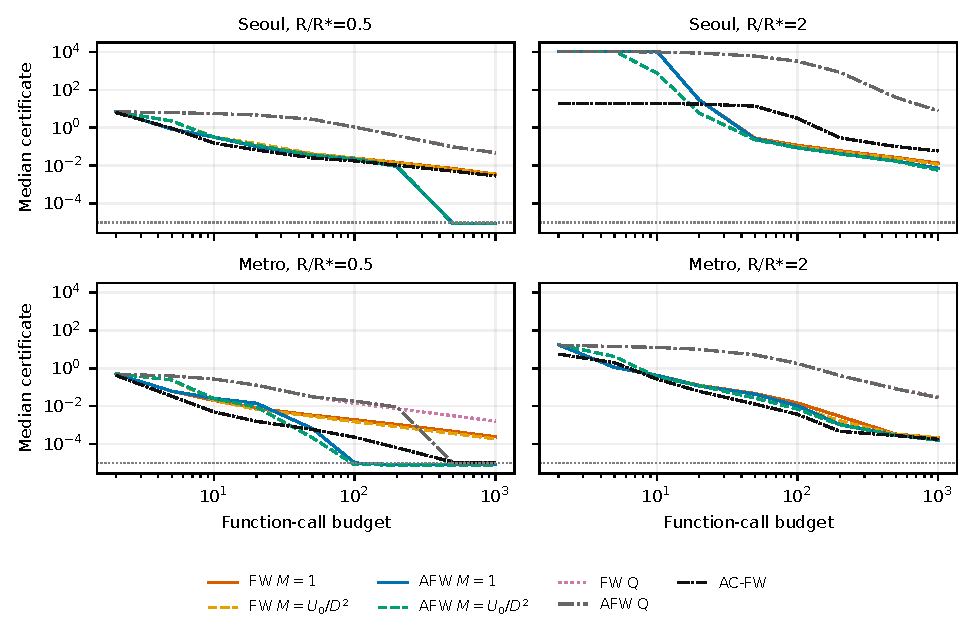
\includegraphics[width=\textwidth]{figures/count_comparators.pdf}
\caption{Median scalar certificates over all distinct vertices at
function-call budgets. Curves include failed runs and charged AC-FW
preprocessing; completed runs are carried forward. The dotted horizontal
line is $10^{-5}$. BT has no curvature inputs, Q receives analytic
$H_0,H_1$. These are paired finite cases, not confidence bands for a
population of problems.}
\label{fig:counts}
\end{figure}

At the active radii, both AFW-BT initializations certify every start at
1000 function calls. FW-BT certifies none on Seoul and only 2/24 or
3/24 on Metro. AC-FW obtains 13/24 active Metro successes and none
on active Seoul. The known-curvature AFW-Q succeeds on all active
Metro starts but none on active Seoul, illustrating conservatism of
the analytic curvature parameters. At the interior radii no method in
this seven-method scalar-certificate comparison reaches the target
within 1000 function calls. End-of-cap results and censored call
medians are reported separately in Table~\ref{tab:counts}.

The references separate remaining error from stopping lag. At the
interior Metro radius, all 24 starts of each BT variant have numerical
reference error upper bound at most $10^{-5}$ by the original endpoint,
but FW has no scalar-certificate successes and AFW has only 6/24 or
7/24. On interior Seoul, the corresponding reference-error condition
holds for 12/30 and 18/30 AFW starts, while neither scalar BT variant
stops. An unsuccessful certificate is therefore not equivalent to a
large remaining primal error.

\subsection{Controlling initialization and objective units}
A separate $2\times2$ study controls the original point versus the
compulsory LMO vertex, and AC versus BT updates. All four cells pay
the same two-source preprocessing, retain both tangent bounds, and
start their first trial at the same secant curvature. Only AC/vertex
is the native published comparator; the other cells isolate factors.
The study contains 280 runs on 70 earlier matched cases and introduces
no new datasets. Table~\ref{tab:init} shows all three planted active
families, including the unfavorable scaled family. Their construction
and the active-face slack identity appear in Appendix~\ref{app:protocol}.

\begin{table}[htbp]
\centering\small
\caption{Starting-point control on three planted active families, ten matched instances each. Counts are certified starts at 1000 function calls. O/V: original point/compulsory initial LMO vertex. The last column is the descriptive paired median BT-V/AC-V certificate ratio and 95\% percentile-bootstrap interval, not a speedup estimate.}
\label{tab:init}
\begin{tabular}{lrrrrl}
\toprule
Family & AC-O & AC-V & BT-O & BT-V & Ratio [interval] \\
\midrule
active & 1 & 10 & 0 & 10 & 1.049 [0.935, 1.257] \\
active\_scaled & 0 & 0 & 0 & 0 & 1.530 [0.822, 1.750] \\
active\_highdim & 6 & 8 & 2 & 8 & 1.231 [0.798, 2.117] \\
\bottomrule
\end{tabular}
\end{table}

On the active family, changing the starting point raises successes
from 1 to 10 for AC and from 0 to 10 for BT. The descriptive
BT/AC certificate-ratio interval from the vertex includes one.
The scaled family remains unsolved by all four controls. Thus the
earlier vertex-start comparison does not isolate an update-rule benefit.

Objective units provide another control. Under $\widetilde f=af+b$,
$a>0$, scaling $M$ and $\varepsilon$ by $a$ preserves the exact
iterates, trials and stopping index, since $G,U,L$ scale together.
Thus $M=U_0/D^2$ is automatically equivariant; fixing its numerical
value instead changes effective initialization. A separate real-data
radius/scale study verifies the counts in all 60 paired scale
comparisons for each certificate-initialized method. This elementary
property does not establish a faster algorithm.

\subsection{Causal stopping controls on fixed BT paths}
We repeat the 432 original BT paths from the count-data study, with
exactly matching original endpoints and oracle counts. Five causal
monitors give 2160 dependent stopping profiles. Disjoint blocks of
$K=8,32,128$ paid affine tangents provide a lower bound using one
additional full LMO per completed block; the scalar envelope is
retained. A separate standard control receives $\mu=0.01$ and uses
$f-\norm{\nabla f}^2/(2\mu)$ as a lower bound. Appendix~\ref{app:monitors}
proves validity and isolated oracle accounting; block sizes are fixed
before outcomes and no monitor reads the reference.

\begin{table}[htbp]
\centering\small
\caption{Isolated causal controls on 432 exactly repeated BT paths, giving 2160 dependent profiles. Counts use each profile's first stop or the original cap. More LMOs compares total direction plus certificate LMOs with scalar. Known $\mu$ receives the analytical ridge coefficient; blocks do not.}
\label{tab:monitors}
\begin{tabular}{lrrr}
\toprule
Profile & Certified & Earlier prefix & More total LMOs \\
\midrule
scalar & 129 & 0 & 0 \\
block\_8 & 129 & 0 & 432 \\
block\_32 & 129 & 0 & 425 \\
block\_128 & 129 & 0 & 380 \\
known\_mu & 226 & 110 & 0 \\
\bottomrule
\end{tabular}
\end{table}

None of the tested blocks gives an earlier stop. The known-$\mu$
control gives 226 successes instead of 129 and 110 earlier prefixes,
with no extra LMOs but additional model information. On interior
Metro each BT variant now reaches 24/24 successes by the original
endpoint; both AFW variants do so within 1000 function calls.
Interior Seoul remains difficult: AFW obtains only 4/30 or 10/30
successes by the endpoint and none at 1000 function calls.
These controls neither establish adaptation to unknown strong convexity
nor evaluate the exact averaged-gradient Fenchel dual in~\cite{pedregosa}.
They show that observable stopping cost is a separate practical issue.


\section{Discussion}
The exposed-face analysis connects the observable FW gap to primal
suboptimality along an actual backtracking trajectory. Normalized atom
weights control the total number of gap-ratio defects, which gives a
local certificate bound without specifying the last exceptional index.
The explicit half-step trajectory separates geometric approach to the
solution face from exact termination. Sparse endpoint probes bridge
that distinction under the full-solution-face and exact-oracle
assumptions.

The loss-dependent curvature model supplies complementary quantitative
bounds. The phase potential accounts for estimates that lag behind
falling curvature and for every rejected function trial; its output is
an observable-certificate guarantee for the existing backtracking rule.
The initialization cost is intrinsic to that halving rule. Positive
$H_1$ on a compact domain is compatible with a global Lipschitz bound,
and the displayed constants can be conservative. At $H_0=0$, the model
itself implies a full exposed solution face; for general positive base
curvature, geometric AFW progress retains its additional gap inequality.

The experiments distinguish initialization, active geometry and
certificate cost. The count-data endpoint controls have nonvertex
optima and lie outside the full-face hypothesis; their unsuccessful
probes quantify overhead. The rational exposed-face example verifies
the termination mechanism on one analytic family. Neither study
establishes a universal empirical advantage. Exact-arithmetic stopping
results also require separate numerical analysis before they can be
used as finite-precision guarantees. The integrated gradient ball gives
a valid optimal-vertex test with certified oracle errors and a separately
charged runner-up margin; it does not establish noisy-algorithm
complexity.

Extending the trajectory argument to controlled inexact directions,
pairwise updates, or more general optimal sets remains open. A separate
question is minimax oracle complexity: the global gradient-dependent
first-order model of~\cite{everest} has different function-class and
initial-distance assumptions. A local compact-domain substitution does
not transfer its lower bounds to the constrained loss-dependent model
and observable LMO certificate considered here.

\begin{thebibliography}{99}
\bibitem{braun} G.~Braun, A.~Carderera, C.~W.~Combettes, H.~Hassani,
A.~Karbasi, A.~Mokhtari, and S.~Pokutta. Conditional Gradient Methods.
\href{https://arxiv.org/abs/2211.14103v5}{arXiv:2211.14103v5}, 2025.
\bibitem{pedregosa} F.~Pedregosa, G.~Negiar, A.~Askari, and M.~Jaggi.
Linearly Convergent Frank-Wolfe with Backtracking Line-Search.
\emph{AISTATS}, 2020. \href{https://arxiv.org/abs/1806.05123}{arXiv:1806.05123}.
\bibitem{lacostejaggi} S.~Lacoste-Julien and M.~Jaggi.
On the Global Linear Convergence of Frank-Wolfe Optimization Variants.
\emph{NeurIPS}, 2015.
\href{https://arxiv.org/abs/1511.05932}{arXiv:1511.05932}.
\bibitem{warmup} F.~Alimisis, R.~Islamov, and A.~Lucchi.
Why Do We Need Warm-up? A Theoretical Perspective.
\href{https://arxiv.org/abs/2510.03164v2}{arXiv:2510.03164v2}, 2026.
\bibitem{kale} S.~Kale, J.~D.~Lee, C.~De~Sa, A.~Sekhari, and K.~Sridharan.
From Gradient Flow on Population Loss to Learning with Stochastic Gradient Descent.
\href{https://arxiv.org/abs/2210.06705v1}{arXiv:2210.06705v1}, 2022.
\bibitem{caoselfbound} D.~Y.~Cao, A.~Y.~Chen, K.~Sridharan, and B.~Tang.
Efficiently Escaping Saddle Points under Generalized Smoothness via Self-Bounding Regularity.
\href{https://arxiv.org/abs/2503.04712v3}{arXiv:2503.04712v3}, 2026.
\bibitem{bomze} I.~M.~Bomze, F.~Rinaldi, and D.~Zeffiro.
Active set complexity of the Away-step Frank-Wolfe Algorithm.
\href{https://arxiv.org/abs/1912.11492}{arXiv:1912.11492}, 2019.
\bibitem{garber} D.~Garber.
Revisiting Frank-Wolfe for Polytopes: Strict Complementarity and Sparsity.
\href{https://arxiv.org/abs/2006.00558}{arXiv:2006.00558}, 2020.
\bibitem{lobanovkoloskova} A.~Lobanov and A.~Koloskova.
Avoiding Bias in Clipped SGD for Overparameterized Models under Generalized Smoothness.
\href{https://arxiv.org/abs/2605.14800v2}{arXiv:2605.14800v2}, 2026.
\bibitem{lobanov} A.~Lobanov.
A Few Accelerated Algorithms for Convex Optimization under $(H_0,H_1)$-Smoothness.
\href{https://arxiv.org/abs/2608.04884}{arXiv:2608.04884}, 2026.
\bibitem{vyguzov} A.~A.~Vyguzov and F.~S.~Stonyakin.
Frank-Wolfe Algorithms for $(L_0,L_1)$-smooth functions.
\href{https://arxiv.org/abs/2510.16468v5}{arXiv:2510.16468v5}, 2026.
\bibitem{selfconcordant} P.~Dvurechensky, K.~Safin, S.~Shtern, and M.~Staudigl.
Generalized Self-Concordant Analysis of Frank-Wolfe Algorithms.
\href{https://arxiv.org/abs/2010.01009}{arXiv:2010.01009}, 2020.
\bibitem{bregmanfw} S.~Takahashi, S.~Pokutta, and A.~Takeda.
Fast Frank--Wolfe Algorithms with Adaptive Bregman Step-Size for Weakly Convex Functions.
\emph{ICLR}, 2026.
\href{https://arxiv.org/abs/2504.04330v4}{arXiv:2504.04330v4}.
\bibitem{adcgs} S.~Takahashi.
Adaptive Conditional Gradient Sliding: Projection-Free and Line-Search-Free Acceleration.
\href{https://arxiv.org/abs/2601.20443v2}{arXiv:2601.20443v2}, 2026.
\bibitem{wirth} E.~Wirth, J.~Pe\~na, and S.~Pokutta.
Fast convergence of Frank-Wolfe algorithms on polytopes.
\href{https://arxiv.org/abs/2406.18789v3}{arXiv:2406.18789v3}, 2025.
\bibitem{restartfw} T.~Kerdreux, A.~d'Aspremont, and S.~Pokutta.
Restarting Frank-Wolfe: Faster Rates under H\"olderian Error Bounds.
\href{https://arxiv.org/abs/1810.02429v4}{arXiv:1810.02429v4}, 2021.
\bibitem{zhao} R.~Zhao.
New Analysis of an Away-Step Frank-Wolfe Method for Minimizing
Logarithmically-Homogeneous Barriers.
\href{https://arxiv.org/html/2305.17808v4}{arXiv:2305.17808v4}, 2023.
\bibitem{autoconditioned} K.-H.~Giang-Tran, S.~Shafiee, and N.~Ho-Nguyen.
Auto-Conditioned Frank-Wolfe Algorithms.
\href{https://arxiv.org/abs/2605.15512}{arXiv:2605.15512}, 2026.
\bibitem{khademi} A.~Khademi and A.~Silveti-Falls.
Adaptive Conditional Gradient Descent.
\href{https://arxiv.org/abs/2510.11440v1}{arXiv:2510.11440v1}, 2025.
\bibitem{yagishita} S.~Yagishita and M.~Ito.
Simple linesearch-free first-order methods for nonconvex optimization.
\href{https://arxiv.org/abs/2509.14670}{arXiv:2509.14670}, 2025.
\bibitem{lacoste2016} S.~Lacoste-Julien.
Convergence Rate of Frank-Wolfe for Non-Convex Objectives.
\href{https://arxiv.org/abs/1607.00345}{arXiv:1607.00345}, 2016.
\bibitem{seoul} Seoul Bike Sharing Demand [Dataset].
UCI Machine Learning Repository, 2020.
\href{https://doi.org/10.24432/C5F62R}{doi:10.24432/C5F62R}. CC BY 4.0.
\bibitem{metro} J.~Hogue. Metro Interstate Traffic Volume [Dataset].
UCI Machine Learning Repository, 2019.
\href{https://doi.org/10.24432/C5X60B}{doi:10.24432/C5X60B}. CC BY 4.0.
\bibitem{karimi} H.~Karimi, J.~Nutini, and M.~Schmidt.
Linear Convergence of Gradient and Proximal-Gradient Methods Under the
Polyak--{\L}ojasiewicz Condition.
\href{https://arxiv.org/abs/1608.04636v4}{arXiv:1608.04636v4}, 2020.
\bibitem{wdbc} W.~Wolberg, O.~Mangasarian, N.~Street, and W.~Street.
Breast Cancer Wisconsin (Diagnostic) [Dataset]. UCI Machine Learning Repository, 1993.
\href{https://doi.org/10.24432/C5DW2B}{doi:10.24432/C5DW2B}.
\bibitem{bike} H.~Fanaee-T. Bike Sharing [Dataset]. UCI Machine Learning Repository, 2013.
\href{https://doi.org/10.24432/C5W894}{doi:10.24432/C5W894}. CC BY 4.0.
\bibitem{liuwarmup} Y.~Liu, Y.~Ge, R.~Pan, K.~An, and T.~Zhang.
Theoretical Analysis on how Learning Rate Warmup Accelerates Convergence.
\href{https://arxiv.org/abs/2509.07972v1}{arXiv:2509.07972v1}, 2025.
\bibitem{freundgrigas} R.~M.~Freund and P.~Grigas.
New Analysis and Results for the Frank-Wolfe Method.
\href{https://arxiv.org/abs/1307.0873}{arXiv:1307.0873}, 2013.
\bibitem{beyondshort} D.~Mart\'inez-Rubio and S.~Pokutta.
Beyond Short Steps in Frank-Wolfe Algorithms.
\href{https://arxiv.org/abs/2501.18773v1}{arXiv:2501.18773v1}, 2025.
\bibitem{alfcg} G.~Yuan.
Adaptive Lipschitz-Free Conditional Gradient Methods for Stochastic
Composite Nonconvex Optimization.
\href{https://arxiv.org/abs/2603.06369v1}{arXiv:2603.06369v1}, 2026.
\bibitem{newtonfw} S.~Takahashi and A.~Takeda.
Beyond Polytopes: Damped Newton Frank--Wolfe Methods over Compact Convex Sets.
\href{https://arxiv.org/abs/2609.34290v1}{arXiv:2609.34290v1}, 2026.
\bibitem{burkeferris} J.~V.~Burke and M.~C.~Ferris.
Weak Sharp Minima in Mathematical Programming.
\emph{SIAM Journal on Control and Optimization}, 31(5):1340--1359, 1993.
\href{https://doi.org/10.1137/0331063}{doi:10.1137/0331063}.
\bibitem{harks} T.~Harks.
Last-Iterate Convergence of Frank--Wolfe for Nonlinear Variational
Inequalities on Polytopes.
\href{https://arxiv.org/abs/2610.17127v1}{arXiv:2610.17127v1}, 2026.
\bibitem{wachsmuth} D.~Wachsmuth and G.~Wachsmuth.
A Simple Proof of the Baillon--Haddad Theorem on Open Subsets of Hilbert
Spaces. \emph{Journal of Convex Analysis}, 30(4):1319--1328, 2023.
\href{https://arxiv.org/abs/2204.00282}{arXiv:2204.00282}.
\bibitem{raj} A.~Raj, J.~Olbrich, B.~G\"artner, B.~Sch\"olkopf, and
M.~Jaggi. Screening Rules for Convex Problems.
\href{https://arxiv.org/abs/1609.07478v1}{arXiv:1609.07478v1}, 2016.
\bibitem{sunbach} Y.~Sun and F.~Bach.
Safe Screening for the Generalized Conditional Gradient Method.
\href{https://arxiv.org/abs/2002.09718v1}{arXiv:2002.09718v1}, 2020.
\bibitem{everest} M.~Rudomanov, I.~Fomin, A.~V.~Gasnikov, and
F.~S.~Stonyakin. Descending Everest with First-Order Oracles: Oracle
Complexity of Convex Optimization under $(L_0,L_1)$-Smoothness.
\href{https://arxiv.org/abs/2610.21461v1}{arXiv:2610.21461v1}, 15 October 2026.
\bibitem{oikonomouloizou} D.~Oikonomou and N.~Loizou.
Curvature-Scaled Sharpness-Aware Minimization: Convergence Beyond
Smoothness. \href{https://arxiv.org/html/2610.29192v1}{arXiv:2610.29192v1},
2026.\end{thebibliography}





\appendix
\section{Comparison steps and certificate normalization}
\label{app:explicit}
If $H_0,H_1$ are supplied, consider
\[
 \alpha=\min\{1,G/[(H_0+H_1U)q^2]\},
\]
with a full step when its curvature is zero.
Lemma~\ref{lem:local}'s descent argument, with $U\ge\delta$,
gives
\[
 f_k-f_{k+1}\ge\frac12\min\{U_k,U_k^2/[D^2(H_0+H_1U_k)]\}.
\]
In a phase $b/2<U\le b$, progress is at least
$\min\{b/4,b^2/(8D^2H_0+4D^2H_1b)\}$, because the right-hand side
is increasing in $U>0$. The phase budget therefore permits at most
$5+4H_1D^2+8H_0D^2/b$ updates. Summing the same dyadic levels proves
\begin{equation}\label{eq:explicitcount}
 N\le\ceil{(5+4H_1D^2)J+16H_0D^2/\varepsilon}.
\end{equation}
There are $N+1$ calls of each oracle for this explicit step.
Exact segment minimization performs at least as well as the comparison
step, so it inherits~\eqref{eq:explicitcount} without receiving
$H_0,H_1$. This does not bound the inner function or gradient calls
needed for an exact scalar minimizer. The expanded technical report
also derives a hyperbolic step with the same order; its elementary
function is not needed for Theorem~\ref{thm:fw}.

For completeness, certificate-scaled backtracking starts with
$\theta_{-1}=1$, tries $\theta_{k-1}/2$, sets $L=\theta U_k/D^2$,
and doubles $\theta$ on a failed quadratic test. The sufficient
threshold $T_k=D^2(H_0/U_k+H_1)$ is nondecreasing. By induction,
\[
 \theta_k\le\max\{2^{-k-1},2T_k\},\qquad
 L_k\le\max\{U_k/(2^{k+1}D^2),2(H_0+H_1U_k)\}.
\]
Indeed a first-trial acceptance halves the previous bound, and after
a rejection the accepted estimate is less than $2T_k$.
Thus $L_k\le2H_0+(2H_1+1/(2D^2))U_k$. Applying the preceding
phase argument with these effective constants gives
\[
 N\le\ceil{(7+8H_1D^2)J+32H_0D^2/\varepsilon}.
\]
The recursion $\theta_k=2^{r_k-1}\theta_{k-1}$ gives
\[
 N_f\le1+2N+\ceil{\log_2\max\{1,2D^2(H_0/\varepsilon+H_1)\}}.
\]
The last source before an update has $U>\varepsilon$, which bounds
$\theta_{N-1}$. This normalization requires $D$ and is optional for
the two-phase order. Theorems~\ref{thm:fw} and~\ref{thm:afw} concern
ordinary backtracking, rather than this separate variant.

\section{Geometric implications and attaining examples}
\label{app:geometry}
Let $p=\inner{\nabla f(x)}{v-s}$ be the pairwise gap over the full
atom set and current active set. The selected FW/away gap is at
least $p/2$. The standard polytope scaling inequality gives, for
any optimal $x^*\ne x$,
\[
 p\ge W\frac{\inner{\nabla f(x)}{x-x^*}}{\norm{x-x^*}}.
\]
See~\cite[Theorem 3]{lacostejaggi} and
\cite[Lemmas 3.4 and 3.6]{restartfw}. For quadratic growth, choose
a nearest optimum. Convexity and the growth inequality imply
$p\ge W\delta/\operatorname{dist}(x,X^*)
\ge W\sqrt{\gamma\delta/2}$. Hence
$g^2\ge\gamma W^2\delta/8$, giving $\kappa=\gamma W^2/16$.
Monotone iterates stay in the initial sublevel set where growth is
assumed. No uniqueness is required. For strong convexity,
$\inner{\nabla f(x)}{x-x^*}\ge\delta+\mu\norm{x-x^*}^2/2$;
minimizing $\delta/r+\mu r/2$ over $r>0$ gives
$p\ge W\sqrt{2\mu\delta}$ and $\kappa=\mu W^2/4$.
These geometric implications are prior results.

\subsection{Gap-envelope equality and zero base curvature}
\label{app:bridge}
\paragraph{The quadratic comparison.}
For $C=D^2(H_0+H_1\delta)$, the feasible step
$t=\min\{1,G/C\}$ and Lemma~\ref{lem:local} give
$\delta\ge G^2/(2C)$ if $G\le C$, and
$\delta\ge G-C/2$ otherwise. The full step is used when $C=0$.
Inverting this established descent inequality gives
\begin{equation}\label{eq:sharpbridge}
 G\le\widehat B(\delta):=
 \begin{cases}\sqrt{2C\delta},&2\delta\le C,\\
 \delta+C/2,&2\delta>C.\end{cases}
\end{equation}
Theorem~\ref{lem:bridge} retains curvature variation along the
segment and strengthens this comparison when $H_1>0$.

\paragraph{Attainment at $H_1=0$.}
Let $Q=[-D/2,D/2]$, $x=D/2$ and $f(y)=h(y-z)^2/2$, $h>0$.
For $z\in Q$, $\delta=h(x-z)^2/2$ and
$G=hD(x-z)=\sqrt{2hD^2\delta}$, attaining the square-root branch
of~\eqref{eq:sharpbridge} with $H_0=h,H_1=0$.
For $z<-D/2$, the constrained optimum is $-D/2$,
$\delta=-hDz$ and $G=\delta+hD^2/2$, attaining its full-step branch.
These examples also attain the $H_1=0$ limit of the exact envelope.

\paragraph{Attainment at $H_1>0$.}
Write $k=\sqrt{H_1}$, $a=kD$, $c=H_0/H_1$, and use $Q=[0,D]$
with source $x=0$. If $c>0$ and
$0<\delta\le c(\cosh a-1)$, set
\[
 r=k^{-1}\operatorname{arcosh}(1+\delta/c),\qquad
 f(u)=c\big(\cosh(k(u-r))-1\big).
\]
This is globally convex, $f_Q^*=f(r)=0$, $f(0)=\delta$,
$f''=H_0+H_1f$, and the source gradient is negative. Thus its
FW atom is $D$ and
$G=-Df'(0)=D\sqrt{2H_0\delta+H_1\delta^2}$.

For $\delta>c(\cosh a-1)$, including all $\delta>0$ when $c=0$,
write $E=E(\delta)$ and, for $u\le D$, set
\[
 f(u)=(\delta+c)\cosh(ku)-\frac{E}{a}\sinh(ku)-c.
\]
On $[0,D]$ it satisfies $f(D)=0$ and
\[
 f'(D)=k\frac{c\cosh a-(\delta+c)}{\sinh a}<0.
\]
The identity $f''=H_0+H_1f$ and this endpoint derivative imply
that $f$ is decreasing and nonnegative on the interval: explicitly,
$f(u)+c=c\cosh(k(D-u))-[f'(D)/k]\sinh(k(D-u))$ for $u\le D$.
It is convex on the entire left half-line. For $u>D$, extend by
\[
 f(u)=f'(D)(u-D)+\tfrac12H_0(u-D)^2.
\]
The two pieces have matching value, derivative and second derivative
at $D$, so the extension is globally convex and $C^2$.
Its constrained optimum is $D$, $f(0)=\delta$, and
$G=-Df'(0)=E$. At $H_0=0$ this becomes
$f(u)=\delta\sinh(k(D-u))/\sinh a$ on $u\le D$, with an affine
extension beyond $D$. These constructions prove optimality for
every parameter tuple, rather than only for the frozen quadratic model.
Since~\eqref{eq:sharpbridge} applies to each attainer, they also
prove $E(\delta)\le\widehat B(\delta)$ and hence that the new
threshold is never smaller than the quadratic one.

\paragraph{An exact global self-bounding corollary.}
The same global inequality and scalar-ray comparison appear in
Oikonomou and Loizou~\cite[Lemma~B.7, Eq.~(30)]{oikonomouloizou}.
We retain this derivation to compare the global model with the
constrained envelope; the global inequality itself is not a new result.
Under the different assumption that the Hessian condition holds on
all of $\R^d$ relative to a finite global infimum $f^*$, one has
\begin{equation}\label{eq:globalselfbound}
 \norm{\nabla f(x)}^2\le2H_0(f(x)-f^*)+H_1(f(x)-f^*)^2.
\end{equation}
Indeed apply the positive-kernel comparison on the entire ray
$x-t\nabla f(x)/\norm{\nabla f(x)}$, $t>0$. Nonnegativity of
$f-f^*$ bounds the initial directional derivative by
\[
 \sqrt{H_1}\inf_{t>0}
 \frac{(f(x)-f^*+H_0/H_1)\cosh(\sqrt{H_1}t)-H_0/H_1}
 {\sinh(\sqrt{H_1}t)}
 =\sqrt{2H_0(f(x)-f^*)+H_1(f(x)-f^*)^2}.
\]
Use the quadratic limit if $H_1=0$, and a limit $t\to\infty$
if $H_0=0<H_1$. The bound is attained by the global cosh objective
above when $H_0,H_1>0$, by a quadratic when $H_1=0<H_0$, and by
$f(x)=A\exp(\sqrt{H_1}x)$, $A>0$, when $H_0=0<H_1$; the latter
infimum is not attained. This gives exact constants for the
global model. The bound in~\cite[Appendix G, Lemma 6]{warmup}
has the larger coefficients $9H_0/4$ and $27H_1/4$; that lemma
does not claim sharpness. For the affine second-order bound,
\cite[Corollary 1]{caoselfbound} instead gives
$\norm{\nabla f}^2\le2(H_0+H_1\delta)^2
\log(1+H_1\delta/H_0)/H_1$ when $H_0,H_1>0$.
The exact polynomial expression in~\eqref{eq:globalselfbound}
removes this logarithmic enlargement. The self-bounding principle
itself is prior work~\cite[Lemma 11]{kale}; only the displayed
constants and extremizers are being compared here, with the exact global
inequality attributed to~\cite{oikonomouloizou}.
The constrained model alone does not
imply~\eqref{eq:globalselfbound}: a nonconstant affine function
on a compact interval has $H_0=H_1=0$ and nonzero gradient.

\paragraph{A polynomial zero-base example.}
The globally convex $C^2$ example $f(x)=t+(\max\{t,0\})^3$,
$t=1/2-x\in[0,1]$ on $Q$, has
$f''(x)=6t\le6f(x)$, so $H_0=0,H_1=6$.
It is not strongly convex. At a nonoptimal interior point both
endpoint atoms are active, and the selected gap is
$(1+3t^2)\max\{t,1-t\}\ge1/2$; the nonoptimal endpoint also satisfies
this inequality. Since $\delta\le2$, condition~\eqref{eq:geometry}
holds with $\kappa=1/16$. At zero error the geometric inequality is
immediate. This shows the $H_0=0$ extension is nonvacuous.

\section{Lower-bound controls and deterministic oracle errors}
\label{app:monitors}
Write $g_j=\nabla f(x_j)$ and $a_j=f(x_j)-\inner{g_j}{x_j}$.
For a completed block $B$ of $K$ consecutive paid sources,
\[
 b_B=\bar a_B+\min_{v\in Q}\inner{\bar g_B}v\le f_Q^*.
\]
Convexity gives $f(v)\ge a_j+\inner{g_j}v$ for each source;
average and minimize to prove validity. Disjoint blocks begin at
source zero, and an incomplete block is not queried. The new lower
bound is the maximum of $\ell_k$ and all completed $b_B$.
Its certificate is nonincreasing and at most $U_k$ on the same
monotone path, so its first crossing occurs no later in updates,
function or gradient calls. At source $k$, exactly
$\lfloor(k+1)/K\rfloor$ additional full LMOs have been performed.
Total LMO cost need not decrease. The monitors affect neither the
line search nor the initial $M$; each reported cost is for one
isolated monitor, excluding the other diagnostic monitors.
An affordable budget source pays its entire scheduled verification.

These uniform block bounds differ from the averaged-gradient Fenchel
dual in~\cite[Theorem 3]{pedregosa}. When the global conjugate exists,
Fenchel equality and Jensen give
\[
 b_B=-\overline{f^*(g_j)}-\sigma_Q(-\bar g_B)
     \le-f^*(\bar g_B)-\sigma_Q(-\bar g_B).
\]
Here $f^*$ denotes the conjugate, not the scalar optimum $f_Q^*$.
No transfer of that paper's theorem or averaging weights is asserted.
With a valid supplied strong-convexity constant $\mu$,
$f(x_j)-\norm{g_j}^2/(2\mu)\le f_Q^*$ follows by minimizing the
quadratic lower model over $\R^d$~\cite[Appendix B]{karimi}.
Caching these bounds costs no LMO, but uses additional information.
Native stopping checks on one synthetic interior instance verify all
20 method/profile pairs against the attainable-prefix construction
and instrument actual oracle calls. They do not represent 2160
additional native solver runs.

\subsection{Certificate validity with bounded deterministic errors}
\label{app:inexact}
If $|\widehat f-f(x)|\le\nu$,
$\norm{\widehat g-\nabla f(x)}\le\rho$ and
$\inner{\widehat g}s\le\min_{v\in Q}\inner{\widehat g}v+\eta$
with known bounds, then
\[
 \ell^{\rm safe}=\widehat f+\inner{\widehat g}{s-x}
                      -\nu-\rho D-\eta\le f_Q^*.
\]
For each $v\in Q$, convexity gives
$f(v)\ge\widehat f-\nu+\inner{\widehat g}{v-x}-\rho D
\ge\ell^{\rm safe}$; minimize over $v$.
A maximum of such lower bounds remains valid, and
$\widehat f+\nu-\max_j\ell_j^{\rm safe}$ is an upper certificate.
This is a validity statement, not a convergence theorem for noisy
directions. Empirical variance is not a deterministic norm bound.

\section{Additional protocol details and controls}
\label{app:protocol}
\paragraph{Features.}
Seoul uses eight numerical weather features (temperature, humidity,
wind speed, visibility, dew point, solar radiation, rainfall and snowfall),
sine/cosine of hour and weekday, holiday and functioning indicators.
Metro uses temperature, rain, snow, cloud cover, sine/cosine of hour,
weekday and day of year (period 365.25), and a holiday indicator.
Other textual categories are omitted. Features constant on training
data are dropped before the $\tanh$ transform; source encodings and
feature names are recorded in the manifests. These deterministic
choices precede the solver comparisons.

\paragraph{Native comparator.}
For $x\ne y$, the AC-FW estimate is
\[
 \ell(x,y)=\frac{2|f(y)-f(x)-\inner{\nabla f(x)}{y-x}|}{\norm{y-x}^2},
\]
and it is zero if $x=y$. Its update is the maximum of this trial estimate
and $r_kL_k$, with $r_k=1-1/((k+1)\log^2(k+3))$.
Only strict objective decrease accepts a trial.
After $N$ outer trials the charged counts are
$N_f=N_{\rm LMO}=N+2$, $N_g=N_{\rm accepted}+2$.
Rejected trials count against the cap. All primary count-data starts
are atoms, as in the cited initialization. Parameter-hidden tests on
both count datasets instrument preprocessing, rejected trials and
oracle calls independently of recorded counters.

\paragraph{Planted geometry.}
For the initialization controls, let
\[
 \phi(x)=m^{-1}\sum_i[\cosh(a_i^\top(x-x^*))-1]
                         +\mu\norm{x-x^*}^2/2,
 \quad f(x)=\phi(x)-\lambda v^\top(x-x^*),
\]
where $\norm{x^*}_1=R$, $v\in\partial\norm{x^*}_1$ and
$\lambda=0.15$. On $Q$, $f\ge\phi\ge0=f_Q^*$ and
$\nabla f(x^*)=-\lambda v\ne0$. Valid constants are
$H_0=\mu+\lambda_{\max}(A^\top A/m)$ and
$H_1=\max_i\norm{a_i}^2$.
The active and active-scaled families use $d=12,m=10$,
$R=1.5,\mu=0.08$, with $x^*$ entries $(0.6,-0.5,0.4)$ at
coordinates $(2,6,10)$; Gaussian row entries have standard deviation
$0.22$ or $0.9$. The high-dimensional family has $d=60,m=40$
and standard deviation $0.22$. Each has ten matched seeds.
Off-support normal coordinates are uniform in $[-0.6,0.6]$.

With $w=\operatorname{sign}(x^*)$, zero off support, the optimal-face
slack $\sigma(x)=R-w^\top x$ obeys
$\sigma(x+\alpha(s-x))=(1-\alpha)\sigma(x)+\alpha\sigma(s)$.
Thus strict subunit steps to atoms on the face keep positive slack
from an exterior start. A full initial vertex move can remove it.
Moreover $f(x)\ge0.4\lambda\sigma(x)$ on these planted examples.
This familiar FW face obstruction explains why initialization is a
necessary control, not a new acceleration mechanism.

\paragraph{Objective-unit study.}
The separate radius/scale archive contains 360 runs on the WDBC
logistic control and UCI Bike Sharing Poisson objective~\cite{wdbc,bike},
three radii, five seeds, three positive scales
and four BT methods. Accuracy is scaled with the objective.
The 60 pairwise scale comparisons per certificate-initialized method
compare final counters and sampled budget certificates, not bitwise
identity of every intermediate iterate. All scalings of a problem
are dependent controls. Additional studies and full baseline settings
are retained in the expanded technical report and companion archive.

\begin{table}[htbp]
\centering\small
\caption{Certification at $10^{-5}$ within 1000 updates. Each cell gives the certified count and median function calls to stop or cap, including failed runs. Seoul has 30 starts and Metro 24 per radius/method. $F/A$: FW/AFW; subscripts $1,U$: BT initialized at $1,U_0/D^2$; $Q$: known-$H$ short step. AC counts 1000 outer trials, including rejections, and pays two preprocessing source evaluations. These medians are not times to success.}
\label{tab:counts}
\begin{tabular}{llrrrrrrr}
\toprule
Data & $R/R_*$ & $F_1$ & $F_U$ & $A_1$ & $A_U$ & $F_Q$ & $A_Q$ & AC \\
\midrule
Seoul & 0.5 & 1; 2001 & 1; 2003 & 30; 424 & 30; 399 & 0; 1001 & 0; 1001 & 0; 1002 \\
Seoul & 2 & 0; 2001 & 0; 1996 & 0; 2001 & 0; 1995.5 & 0; 1001 & 0; 1001 & 0; 1002 \\
Metro & 0.5 & 3; 2001 & 3; 2003 & 24; 99 & 24; 80.5 & 1; 1001 & 24; 423 & 13; 385 \\
Metro & 2 & 0; 2000 & 0; 2002 & 6; 2000 & 7; 2001 & 0; 1001 & 0; 1001 & 0; 1002 \\
\bottomrule
\end{tabular}
\end{table}


\section{What the closest bounds directly establish}
\label{app:comparison}
The following comparison concerns specific stated results, not every
possible consequence of their proofs.
Khademi and Silveti-Falls~\cite[Theorems 4.4--4.5]{khademi}
combine gradient-difference estimates with backtracking. Their stated
constrained rates retain a global smoothness/gradient contribution;
they also explicitly discuss slow downward adaptation of ordinary
backtracking. Thus that motivation is prior. Yagishita and
Ito~\cite[Algorithm 3, Theorem 3.1]{yagishita} analyze a line-search-free
composite conditional-gradient method with a nondecreasing estimate
and a nonconvex minimum-gap guarantee. These are different methods
and stopping statements, not evidence for a general priority claim.
Pedregosa et al.~\cite[Theorem 3]{pedregosa} bound a last-iterate
Fenchel primal--dual gap using averaged accepted curvature estimates.
Its dual lower value and the maximum scalar tangent lower bound have
no general ordering for arbitrary histories: for $f=x^2/2$ on
$[-1,1]$, histories $(-1,1)$ and $(-1,-1/2)$ reverse the order.
These histories are not asserted to be algorithm trajectories and do
not contradict that theorem. Its Theorem 4 already yields geometric
progress from accepted local curvature, which our AFW proof specializes.

Substituting $L_Q=H_0+H_1\max_Q\delta$ in a global smoothness bound
retains the global gap range. The smaller initial certificate $U_0$
does not bound curvature everywhere on $Q$; restricting the region
to an initial sublevel set would change its LMO.
Our first-return argument instead bounds only the tested descent
segment. A phase count controls estimates above the current level.

The deterministic convex result in~\cite[Appendix C.4]{lobanovkoloskova}
already separates function-dependent-curvature regimes for gradient
descent; it is not an LMO certificate theorem.
The gradient-norm dependent FW analysis in~\cite[Theorem 5.1]{vyguzov}
contains a largest-gradient contribution after a direct substitution.
Neither the use of phases nor unknown-curvature adaptation alone
is presented as new here.

Takahashi et al.~\cite{bregmanfw} use relative smoothness, a kernel,
and segment scaling. A Euclidean kernel with a single global $L_Q$
does not by itself give the separated dependence above.
For adaptive sliding~\cite[Theorems 2.1 and 4.1]{adcgs}, inner LMO
effort is distinct from outer iterations, and the restarted theorem
also requires local strong convexity and its scheduling parameters.
Condition~\eqref{eq:curvature} alone does not give strong convexity:
$\cosh(x_1)-1$ on a square has a line of minimizers.
No superiority over sliding is established.

Wirth et al.~\cite[Definition 2.3(b), Theorem 3.6]{wirth} use uniform
extended curvature and a vertex error bound. Kerdreux et
al.~\cite[Proposition 4.2, Theorem 5.1]{restartfw} already combine
burn-in, computable strong-Wolfe stopping, unknown error-bound
parameters and cumulative LMO counts, with global away curvature.
Zhao~\cite[Theorems 4.1--4.2]{zhao} proves linear objective- and
FW-gap rates for log-homogeneous barriers, using exact search or a
local-Hessian step. Our function class and the evaluated algorithm
differ. None of these comparisons rules out an equivalent refined
specialization of another adaptive proof.

Generalized self-concordant FW~\cite{selfconcordant} uses a different
curvature model and corresponding step rules. Yuan~\cite{alfcg} studies
stochastic composite nonconvex optimization under component or average
smoothness assumptions and a stationarity criterion. The damped
Newton--FW method of~\cite{newtonfw} uses Hessian information and
positive definite Hessians, whereas the zero-base optimum here has a
vanishing Hessian. These statements concern the specified models and
algorithms, not a general impossibility of deriving refined consequences
from earlier analyses.

\section{Reproducibility and evidence checks}
\label{app:reproduction}
The companion package includes source snapshots, raw data attribution,
CSV results and SHA-256 manifests. The main real-data comparison
joins 648 preserved records with 108 additional AC-FW records on the
same cases; it does not count them as new datasets.
The certificate study replays 432 existing paths and reports 2160
dependent causal profiles. The initialization factorial also reuses
earlier cases. Table values are generated from immutable CSVs; the
claim ledger records each selection and its value.

The baseline records use Python 3.13.5, NumPy 2.5.2, SciPy 1.16.3,
Matplotlib 3.10.9 and scikit-learn 1.8.0, with BLAS/OpenMP thread
environment variables set to one. The endpoint-probe protocol uses
Python 3.13.5, NumPy 2.3.5 and SciPy 1.16.3; its manifest records the
versions and thread settings. From the repository root, the regression
suite is run with
\begin{verbatim}
python -m unittest discover -s PART3/Work -p "test_*.py"
\end{verbatim}
The regression tests cover derivatives, reference independence, actual oracle
calls, certificates, accepted progress and curvature limits. Full
trajectory audits run before trace sampling; saved validators also
check provenance and budget accounting.
A separate finite audit uses exact rational arithmetic for 8370
phase configurations, 57989 abstract curvature-state visits, phase
budgets, gap inversion and atom-removal counts. It overapproximates
possible curvature histories and does not assert that every state
is realizable by an objective. Finite tests are not a formal proof
or independent mathematical review.

Further tests cover the exact differential envelope, its
inverse and large-parameter limits, one-dimensional extremizers in
70-digit decimal arithmetic, and actual gaps on five earlier synthetic
and regression objectives. A separate rational archive contains 24
AFW runs from uniform atom weights on simplex and box examples, six planted
local states (12 maximal drops), and 180 quadratic trial checks for
the positive-base counterexample. All 30 zero-base runs reach an
exact zero objective and certificate. These are finite algebraic
checks of the stated mechanisms, not evidence of a uniform empirical
speedup. Both exact-audit archives replay from their own saved code.

For the simplex examples $t=c^\top x$, $c=(0,0,1,2)$, and
$f=t+\beta t^3$, $\beta\in\{0,1/16,1\}$. The Hessian norm is
$6\beta t\norm c^2=30\beta t\le30\beta f$ on the simplex.
For the box $0\le t\le1$, $|y|\le1/2$, use
$f=t+\beta t^3(1+y^2)$. Its Hessian has nonnegative diagonal and
determinant $12\beta^2t^4(1-2y^2)\ge0$; its norm is at most its
trace, $6\beta t(1+y^2)+2\beta t^3\le(19\beta/2)t\le10\beta f$.
Both families have a non-singleton exposed optimal face and atom
margin $m=1$. Replacing $t^3$ by $(\max\{t,0\})^3$ supplies a
convex $C^2$ extension to a neighborhood without changing any feasible
value. The four initial estimates are $1/4,1,4,64$. Planted local
states retain two optimal and two nonoptimal atoms and terminate by
two exact maximal away steps.
Two further rational paths in the tests start near that face with
$M=65536$, giving respectively seven and eight nonmaximal away
updates before their last two drops. They exercise the separate
initialization potential $Q_0$ in Theorem~\ref{thm:zerofinite}.

The broader baseline experiments include repeated Bike Sharing initial
vertices: ten seed indices give seven distinct starts. Later
activity-sweep summaries explicitly remove those duplicates. Those
seed-weighted summaries are not used as independent
replications in the main count-data comparison, which enumerates all
distinct vertices. Numerical references and floating-point audits
do not provide directed-rounding guarantees.

\paragraph{Limited formal algebra checks.}
The limited algebra file \texttt{ResearchAlgebra.lean} compiles under
Lean 4.35.0-rc2 using only its core/Std library. It checks two generic
commutative-ring identities after clearing denominators and seven closed
integer identities or inequalities for the exact examples. Its axiom
audit uses only Lean's standard logical axioms for the generic identities;
the closed checks are axiom-free. These small checks do not formalize
the analytic trajectory, complexity, or vertex-identification theorems.

\paragraph{Generative-tool disclosure.}
An OpenAI Codex assistant was used substantially for literature triage,
proof development, implementation, experiment analysis, manuscript
drafting and verification automation. The explicit derivations, source
snapshots and executable checks are supplied for scrutiny. Automated
checks and AI-assisted internal review are not independent mathematical
peer review. Responsibility for the submitted scientific claims rests
with the named authors.

\section{Endpoint probes with a persistent vertex cache}
\label{app:endpoint}
The finite-termination result of Corollary~\ref{face:endpoint} does not
imply a practical advantage outside its full-solution-face assumptions.
We evaluated 108 matched dataset/radius/start configurations from the
Seoul and Metro count-data tasks with three methods: ordinary
backtracking, endpoint tests at every update, and tests at indices
$k+1=2^j$, $j=0,1,\ldots$. These are configurations from two datasets,
not independent statistical samples. All methods start from the same
source and use $M=U_0/D^2$; the endpoint Armijo coefficient is
$\sigma=1/2$.

\paragraph{Persistent cache and paid-budget protocol.}
Each method, including its ordinary baseline, has its own persistent
cache. Only values at exactly represented signed-coordinate vertices
are shared between queries: the cache key records dimension, coordinate
and sign, and membership requires exact coordinate equality to the
radius and exact zeros elsewhere. Nearby points do not share a key.
The deterministic Float64 objective and operation order are fixed;
cache hits reuse that value without another paid function call.
Nonvertex values, gradients and full LMOs remain separately charged.
A failed endpoint test uses the unchanged quadratic-backtracking
fallback and tie rule. At the budget of 1000 paid objective calls, the
reported source prefix is the last source whose cumulative paid
function count is at most 1000; a trial that crosses the budget does
not make the subsequent source affordable. Other oracle types are
unrestricted in this single-oracle comparison.

\begin{table}[htbp]
\centering
\small
\caption{Persistent-cache endpoint probes: certificate ratio $U_{\rm probe}/U_{\rm ordinary}$ at 1000 paid objective evaluations, over 108 paired configurations.}
\label{endpoint:table}
\begin{tabular}{lrrrr}
\toprule
Probe schedule & Median ratio & Better $>1\%$ & Worse $>1\%$ & Within $1\%$ \\
\midrule
Dense & 1.004798 & 0 & 35 & 73 \\
Dyadic & 1.000727 & 0 & 12 & 96 \\
\bottomrule
\end{tabular}
\end{table}


No endpoint test was accepted in any of the 324 runs. At the common
1000-call source prefix, the dense persistent-cache median certificate
ratio was $1.00479805149$; 0, 35 and 73 configurations were respectively
better by more than 1\%, worse by more than 1\%, and within 1\% of the
ordinary baseline. The corresponding dyadic median was $1.00072704517$,
with counts 0, 12 and 96. A paired audit of the 216 dense/dyadic versus
ordinary paths found 106623 matching sources and 106407 matching
transitions, including objective, gap, certificate, accepted curvature
and step. At equal update counts, every paid-function difference was
between zero and the number of vertices; the maximum observed extra
cost was 17 calls.

Ridge regularization makes the Poisson objective strictly convex.
In every task, numerical comparison placed each vertex above a better
feasible reference point, locating the unique optimum away from the
vertices. These tasks
therefore do not satisfy~\eqref{face:exposed}; in particular, their
minimizers do not form the full exposed solution face assumed by the
termination theorem. The results measure the cost of unsuccessful
probes outside that regime. They establish neither a wall-clock speedup
nor better progress per mathematical update.

\paragraph{A cache bound at equal update counts.}
If all added probes are rejected, the initial state and fallback rule
coincide, and both methods permanently cache exact vertex values, then
for every fixed number $K$ of updates,
\[
 0\le N_f^{\rm probe}(K)-N_f^{\rm ordinary}(K)\le |V|.
\]
Indeed, all fallback iterates and nonvertex queries coincide. Each
vertex is paid for at most once, and the difference counts vertices
queried only by the probing method. This statement concerns equal
update counts; Table~\ref{endpoint:table} instead fixes a paid-function
budget.

\subsection{An exact check within the exposed-face assumptions}
\paragraph{An exposed-face mechanism check.}
To complement the out-of-regime count-data controls, we independently
implemented the exact example of Section~5.1 using rational arithmetic.
The study contains 54 exact runs: six ordinary baseline runs and 48
endpoint-probe runs. The six starts use
$t_0\in\{1,1/2,1/4\}$ and $z_0\in\{-1/3,1/3\}$. The probe runs
vary over $\sigma\in\{1/2,9/10,99/100,1-2^{-20}\}$ and dense or
dyadic schedules. Ordinary FW remains nonterminal at the
64-update audit cap; the manuscript's analytic recurrence describes
its infinite continuation. All 48 probing runs attain $U=0$ exactly,
within at most 16 updates. The 222 sources preceding an accepted
endpoint match their ordinary counterparts exactly in iterate,
objective, gap and scalar certificate. A persistent cache pays for at
most two distinct endpoint values in these runs. These are variations
of one analytic example, not independent datasets or evidence of a
general practical advantage. Source, full traces and a SHA-256 manifest
are supplied in the companion archive.

\begin{figure}[htbp]
\centering
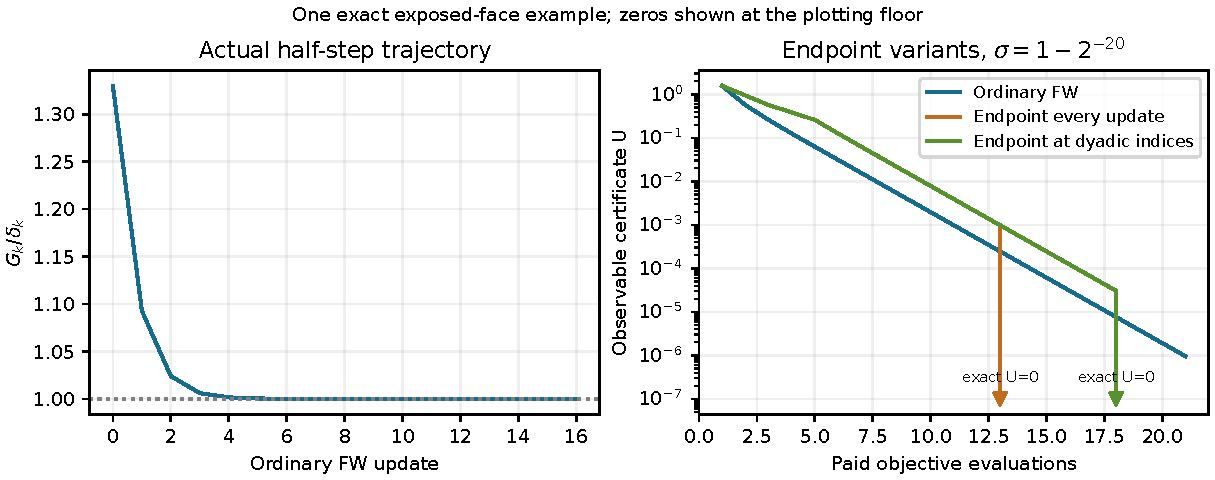
\includegraphics[width=\textwidth]{figures/exposed_face_mechanism.pdf}
\caption{Exact exposed-face study with 54 runs: six ordinary baselines
and 48 dense or dyadic endpoint-probe runs. Left: the half-step
trajectory has $G_k/\delta_k\to1$. Right: dense and dyadic endpoint
tests reach exact $U=0$; zeros are marked at a display floor of
$10^{-7}$. The ordinary run remains nonterminal. The horizontal axis
counts paid objective evaluations; this illustration does not give a
general practical ranking. Source, traces and SHA-256 manifest are
available in the companion archive.}
\label{fig:face-mechanism}
\end{figure}


\end{document}
